% Options for packages loaded elsewhere
\PassOptionsToPackage{unicode}{hyperref}
\PassOptionsToPackage{hyphens}{url}
\documentclass[
  11pt,
]{article}
\usepackage{xcolor}
\usepackage[margin=2.5cm]{geometry}
\usepackage{amsmath,amssymb}
\setcounter{secnumdepth}{5}
\usepackage{iftex}
\ifPDFTeX
  \usepackage[T1]{fontenc}
  \usepackage[utf8]{inputenc}
  \usepackage{textcomp} % provide euro and other symbols
\else % if luatex or xetex
  \usepackage{unicode-math} % this also loads fontspec
  \defaultfontfeatures{Scale=MatchLowercase}
  \defaultfontfeatures[\rmfamily]{Ligatures=TeX,Scale=1}
\fi
\usepackage{lmodern}
\ifPDFTeX\else
  % xetex/luatex font selection
  \setmainfont[]{Arial}
\fi
% Use upquote if available, for straight quotes in verbatim environments
\IfFileExists{upquote.sty}{\usepackage{upquote}}{}
\IfFileExists{microtype.sty}{% use microtype if available
  \usepackage[]{microtype}
  \UseMicrotypeSet[protrusion]{basicmath} % disable protrusion for tt fonts
}{}
\makeatletter
\@ifundefined{KOMAClassName}{% if non-KOMA class
  \IfFileExists{parskip.sty}{%
    \usepackage{parskip}
  }{% else
    \setlength{\parindent}{0pt}
    \setlength{\parskip}{6pt plus 2pt minus 1pt}}
}{% if KOMA class
  \KOMAoptions{parskip=half}}
\makeatother
\usepackage{color}
\usepackage{fancyvrb}
\newcommand{\VerbBar}{|}
\newcommand{\VERB}{\Verb[commandchars=\\\{\}]}
\DefineVerbatimEnvironment{Highlighting}{Verbatim}{commandchars=\\\{\}}
% Add ',fontsize=\small' for more characters per line
\usepackage{framed}
\definecolor{shadecolor}{RGB}{248,248,248}
\newenvironment{Shaded}{\begin{snugshade}}{\end{snugshade}}
\newcommand{\AlertTok}[1]{\textcolor[rgb]{0.94,0.16,0.16}{#1}}
\newcommand{\AnnotationTok}[1]{\textcolor[rgb]{0.56,0.35,0.01}{\textbf{\textit{#1}}}}
\newcommand{\AttributeTok}[1]{\textcolor[rgb]{0.13,0.29,0.53}{#1}}
\newcommand{\BaseNTok}[1]{\textcolor[rgb]{0.00,0.00,0.81}{#1}}
\newcommand{\BuiltInTok}[1]{#1}
\newcommand{\CharTok}[1]{\textcolor[rgb]{0.31,0.60,0.02}{#1}}
\newcommand{\CommentTok}[1]{\textcolor[rgb]{0.56,0.35,0.01}{\textit{#1}}}
\newcommand{\CommentVarTok}[1]{\textcolor[rgb]{0.56,0.35,0.01}{\textbf{\textit{#1}}}}
\newcommand{\ConstantTok}[1]{\textcolor[rgb]{0.56,0.35,0.01}{#1}}
\newcommand{\ControlFlowTok}[1]{\textcolor[rgb]{0.13,0.29,0.53}{\textbf{#1}}}
\newcommand{\DataTypeTok}[1]{\textcolor[rgb]{0.13,0.29,0.53}{#1}}
\newcommand{\DecValTok}[1]{\textcolor[rgb]{0.00,0.00,0.81}{#1}}
\newcommand{\DocumentationTok}[1]{\textcolor[rgb]{0.56,0.35,0.01}{\textbf{\textit{#1}}}}
\newcommand{\ErrorTok}[1]{\textcolor[rgb]{0.64,0.00,0.00}{\textbf{#1}}}
\newcommand{\ExtensionTok}[1]{#1}
\newcommand{\FloatTok}[1]{\textcolor[rgb]{0.00,0.00,0.81}{#1}}
\newcommand{\FunctionTok}[1]{\textcolor[rgb]{0.13,0.29,0.53}{\textbf{#1}}}
\newcommand{\ImportTok}[1]{#1}
\newcommand{\InformationTok}[1]{\textcolor[rgb]{0.56,0.35,0.01}{\textbf{\textit{#1}}}}
\newcommand{\KeywordTok}[1]{\textcolor[rgb]{0.13,0.29,0.53}{\textbf{#1}}}
\newcommand{\NormalTok}[1]{#1}
\newcommand{\OperatorTok}[1]{\textcolor[rgb]{0.81,0.36,0.00}{\textbf{#1}}}
\newcommand{\OtherTok}[1]{\textcolor[rgb]{0.56,0.35,0.01}{#1}}
\newcommand{\PreprocessorTok}[1]{\textcolor[rgb]{0.56,0.35,0.01}{\textit{#1}}}
\newcommand{\RegionMarkerTok}[1]{#1}
\newcommand{\SpecialCharTok}[1]{\textcolor[rgb]{0.81,0.36,0.00}{\textbf{#1}}}
\newcommand{\SpecialStringTok}[1]{\textcolor[rgb]{0.31,0.60,0.02}{#1}}
\newcommand{\StringTok}[1]{\textcolor[rgb]{0.31,0.60,0.02}{#1}}
\newcommand{\VariableTok}[1]{\textcolor[rgb]{0.00,0.00,0.00}{#1}}
\newcommand{\VerbatimStringTok}[1]{\textcolor[rgb]{0.31,0.60,0.02}{#1}}
\newcommand{\WarningTok}[1]{\textcolor[rgb]{0.56,0.35,0.01}{\textbf{\textit{#1}}}}
\usepackage{longtable,booktabs,array}
\newcounter{none} % for unnumbered tables
\usepackage{calc} % for calculating minipage widths
% Correct order of tables after \paragraph or \subparagraph
\usepackage{etoolbox}
\makeatletter
\patchcmd\longtable{\par}{\if@noskipsec\mbox{}\fi\par}{}{}
\makeatother
% Allow footnotes in longtable head/foot
\IfFileExists{footnotehyper.sty}{\usepackage{footnotehyper}}{\usepackage{footnote}}
\makesavenoteenv{longtable}
\usepackage{graphicx}
\makeatletter
\newsavebox\pandoc@box
\newcommand*\pandocbounded[1]{% scales image to fit in text height/width
  \sbox\pandoc@box{#1}%
  \Gscale@div\@tempa{\textheight}{\dimexpr\ht\pandoc@box+\dp\pandoc@box\relax}%
  \Gscale@div\@tempb{\linewidth}{\wd\pandoc@box}%
  \ifdim\@tempb\p@<\@tempa\p@\let\@tempa\@tempb\fi% select the smaller of both
  \ifdim\@tempa\p@<\p@\scalebox{\@tempa}{\usebox\pandoc@box}%
  \else\usebox{\pandoc@box}%
  \fi%
}
% Set default figure placement to htbp
\def\fps@figure{htbp}
\makeatother
\setlength{\emergencystretch}{3em} % prevent overfull lines
\providecommand{\tightlist}{%
  \setlength{\itemsep}{0pt}\setlength{\parskip}{0pt}}
\usepackage{fancyhdr}
\pagestyle{fancy}
% Ne pas inclure de logos dans l'en-tête par défaut
\fancyhead{}
% Vous pouvez conserver le pied de page avec le numéro de page si vous le souhaitez
\fancyfoot[C]{\thepage}
% Assurez-vous que la hauteur de l'en-tête est correcte
\setlength{\headheight}{15pt}
\usepackage{booktabs}
\usepackage{longtable}
\usepackage{array}
\usepackage{multirow}
\usepackage{wrapfig}
\usepackage{float}
\usepackage{colortbl}
\usepackage{pdflscape}
\usepackage{tabu}
\usepackage{threeparttable}
\usepackage{threeparttablex}
\usepackage[normalem]{ulem}
\usepackage{makecell}
\usepackage{xcolor}
\usepackage{bookmark}
\IfFileExists{xurl.sty}{\usepackage{xurl}}{} % add URL line breaks if available
\urlstyle{same}
\hypersetup{
  hidelinks,
  pdfcreator={LaTeX via pandoc}}

\author{}
\date{\vspace{-2.5em}}

\begin{document}

\begin{titlepage}
\begin{center}

\begin{minipage}{0.15\textwidth}

\includegraphics[width=\linewidth]{logo_ansd}
\end{minipage}
\hfill
\begin{minipage}{0.15\textwidth}

\includegraphics[width=\linewidth]{logo_ensae}
\end{minipage}

\vspace{2cm}

{\Huge\bfseries TP3 : Accès aux services de santé et chocs sanitaires des ménages \par}
\vspace{1.5cm}

{\Large\textbf{Rapport d'analyse}}\par
\vspace{1.5cm}

\textbf{Auteurs :}\par
\vspace{0.5cm}
Mouhamet SECK\\
\vspace{0.2cm}
Manampisoa Clarrat FINARITRINIAINA\\

\vfill

{\Large Projet statistique avec R ou python}\\
\vspace{1cm}
{\large ENSAE - ISE1-CL / ISE1 MATH - Mars 2026}

\vspace{1cm}

\end{center}
\end{titlepage}

{
\setcounter{tocdepth}{2}
\tableofcontents
}
\newpage

\section{Introduction}\label{introduction}

Ce rapport présente les analyses descriptives et les tests statistiques
réalisés dans le cadre du TP3, à partir des données de la Nigeria
General Household Survey (GHS) Panel -- vague 2 (2012--2013). L'objectif
est d'étudier la morbidité, le recours aux soins, les dépenses de santé,
et leurs liens avec les caractéristiques démographiques et le niveau de
vie des ménages.

\subsection{Justification du choix de la vague
2}\label{justification-du-choix-de-la-vague-2}

Initialement, le TP devait exploiter la vague 4. Cependant, après examen
des fichiers disponibles :

\begin{itemize}
\item
  Les fichiers \texttt{sect3a\_harvestw4} et \texttt{sect3b\_harvestw4}
  correspondent en réalité au module \textbf{Travail} et non au module
  santé.
\item
  Le fichier de consommation \texttt{cons\_agg\_wave4\_visit2} est
  absent.
\end{itemize}

En revanche, pour la vague 2 nous disposons de :

\begin{itemize}
\item
  \texttt{sect4a\_harvestw2.dta} : module santé complet (morbidité,
  recours aux soins, dépenses)
\item
  \texttt{sect1\_harvestw2.dta} : données démographiques (sexe, âge,
  milieu de résidence)
\item
  \texttt{cons\_agg\_wave2\_visit2.dta} : agrégats de consommation
  (niveau de vie)
\end{itemize}

Toutes les analyses ont donc été réalisées sur cette vague, garantissant
la disponibilité et la cohérence des informations nécessaires.

\section{Méthodologie}\label{muxe9thodologie}

\subsection{Données et Variables
Clés}\label{donnuxe9es-et-variables-cluxe9s}

Les fichiers suivants ont été utilisés :

\begin{itemize}
\item
  \textbf{sect4a\_w2} : 27 363 individus, variables de santé (morbidité,
  consultations, dépenses).
\item
  \textbf{sect1\_w2} : 30 234 individus, variables démographiques (sexe,
  âge, secteur urbain/rural).
\item
  \textbf{cons\_w2} : 4 738 ménages, consommation totale
  (\texttt{totcons}) servant à construire les quintiles de niveau de
  vie.
\end{itemize}

Les variables clés retenues sont :

\begin{itemize}
\item
  \textbf{Morbidité} : \texttt{s4aq3} (1 = maladie, 2 = blessure, 3 =
  aucun problème).
\item
  \textbf{Recours aux soins} : \texttt{s4aq6a} (premier prestataire
  consulté) et \texttt{s4aq1} (consultation ou non).
\item
  \textbf{Dépenses de santé} : \texttt{s4aq9} (coût consultation),
  \texttt{s4aq14} (médicaments OTC), \texttt{s4aq17} (hospitalisation),
  \texttt{s4aq19} (autres médicaments).
\item
  \textbf{Caractéristiques individuelles} : \texttt{s1q2} (sexe),
  \texttt{s1q4} (âge), \texttt{sector} (1 = urbain, 2 = rural).
\item
  \textbf{Niveau de vie} : \texttt{totcons} (consommation totale par
  équivalent adulte).
\end{itemize}

\subsection{Traitements Effectués}\label{traitements-effectuuxe9s}

\begin{Shaded}
\begin{Highlighting}[]
\CommentTok{\# Jointure des fichiers santé et démographie}
\NormalTok{data }\OtherTok{\textless{}{-}} \FunctionTok{left\_join}\NormalTok{(sect4a\_w2, sect1\_w2, }\AttributeTok{by =} \FunctionTok{c}\NormalTok{(}\StringTok{"hhid"}\NormalTok{, }\StringTok{"indiv"}\NormalTok{))}

\CommentTok{\# Création de variables}
\NormalTok{data }\OtherTok{\textless{}{-}}\NormalTok{ data }\SpecialCharTok{\%\textgreater{}\%}
  \FunctionTok{mutate}\NormalTok{(}
    \AttributeTok{morbidite  =} \FunctionTok{ifelse}\NormalTok{(s4aq3 }\SpecialCharTok{\%in\%} \FunctionTok{c}\NormalTok{(}\DecValTok{1}\NormalTok{, }\DecValTok{2}\NormalTok{), }\DecValTok{1}\NormalTok{, }\DecValTok{0}\NormalTok{),}
    \AttributeTok{groupe\_age =} \FunctionTok{cut}\NormalTok{(s1q4, }\AttributeTok{breaks =} \FunctionTok{c}\NormalTok{(}\DecValTok{0}\NormalTok{, }\DecValTok{14}\NormalTok{, }\DecValTok{30}\NormalTok{, }\DecValTok{45}\NormalTok{, }\DecValTok{60}\NormalTok{, }\ConstantTok{Inf}\NormalTok{),}
                     \AttributeTok{labels =} \FunctionTok{c}\NormalTok{(}\StringTok{"\textless{}15"}\NormalTok{, }\StringTok{"15{-}30"}\NormalTok{, }\StringTok{"31{-}45"}\NormalTok{, }\StringTok{"46{-}60"}\NormalTok{, }\StringTok{"61+"}\NormalTok{)),}
    \AttributeTok{dep\_totale =} \FunctionTok{rowSums}\NormalTok{(}\FunctionTok{cbind}\NormalTok{(s4aq9, s4aq14, s4aq17, s4aq19), }\AttributeTok{na.rm =} \ConstantTok{TRUE}\NormalTok{),}
    \AttributeTok{consulte   =} \FunctionTok{ifelse}\NormalTok{(}\SpecialCharTok{!}\FunctionTok{is.na}\NormalTok{(s4aq6a), }\DecValTok{1}\NormalTok{, }\DecValTok{0}\NormalTok{)}
\NormalTok{  )}

\CommentTok{\# Calculs : taux de morbidité avec intervalles de confiance (méthode binomiale exacte)}

\CommentTok{\# Tests statistiques :}
\CommentTok{\#   {-} Chi{-}deux d\textquotesingle{}indépendance entre recours aux soins et quintile de consommation}
\CommentTok{\#   {-} V de Cramér pour mesurer l\textquotesingle{}intensité de l\textquotesingle{}association}
\CommentTok{\#   {-} Test de Wilcoxon{-}Mann{-}Whitney pour comparer les dépenses rural / urbain}
\end{Highlighting}
\end{Shaded}

Les traitements réalisés comprennent la jointure des fichiers santé et
démographie sur les identifiants ménage (\texttt{hhid}) et individu
(\texttt{indiv}), la création de variables (morbidité binaire, groupes
d'âge, dépense totale de santé, indicateur de consultation), ainsi que
des calculs de taux de morbidité global et par sous-groupe avec
intervalles de confiance (méthode binomiale exacte). Des tests
statistiques ont également été effectués : chi-deux d'indépendance entre
recours aux soins et quintile de consommation, V de Cramér pour mesurer
l'intensité de l'association, et test de Wilcoxon-Mann-Whitney pour
comparer les dépenses de santé entre milieux rural et urbain. Des
visualisations ont été produites : barplots, histogrammes, boxplots,
violin plots, barplots 100 \% empilés.

\section{Résultats}\label{ruxe9sultats}

\subsection{Qualité des Données et Valeurs
Manquantes}\label{qualituxe9-des-donnuxe9es-et-valeurs-manquantes}

L'examen des valeurs manquantes sur nos variables d'intérêt révèle une
situation globalement satisfaisante. Dans le fichier \texttt{cons\_w2},
la variable totcons ainsi que toutes les variables de consommation
alimentaire et non alimentaire ne présentent aucune valeur manquante,
garantissant l'intégrité des quintiles de niveau de vie construits. Dans
\texttt{sect1\_w2}, les variables clés retenues (\texttt{s1q2} (sexe),
\texttt{s1q4} (âge, 3,55 \%) et sector (milieu, 0 \%)) sont quasi
exhaustives, avec un taux de manquants négligeable pour l'âge. Dans
\texttt{sect4a\_w2}, les variables \texttt{s4aq3} (morbidité, 0,87 \%),
s4aq1 (consultation, 0,72 \%) et s4aq6a (prestataire, 88,18 \%)
présentent des profils attendus : le fort taux de manquants sur
\texttt{s4aq6a} est structurel, car seuls les individus ayant
effectivement consulté devaient renseigner cette variable. Les variables
de dépenses (\texttt{s4aq9}, \texttt{s4aq14}, \texttt{s4aq17},
\texttt{s4aq19}) affichent de même des taux élevés (65 - 89 \%),
cohérents avec leur caractère conditionnel à une consultation ou un
achat.

\subsection{Taux de Morbidité}\label{taux-de-morbidituxe9}

Le taux de morbidité (maladie ou blessure au cours des 4 dernières
semaines) est de \textbf{12,2 \%} (IC 95 \% : {[}11,8 \% -- 12,6 \%{]}).

\begin{longtable}[]{@{}lrrrrr@{}}
\caption{Taux de morbidité global}\tabularnewline
\toprule\noalign{}
indicateur & effectif & cas & proportion & ic\_inf & ic\_sup \\
\midrule\noalign{}
\endfirsthead
\toprule\noalign{}
indicateur & effectif & cas & proportion & ic\_inf & ic\_sup \\
\midrule\noalign{}
\endhead
\bottomrule\noalign{}
\endlastfoot
Taux de morbidité global & 27126 & 3309 & 0.122 & 0.118 & 0.126 \\
\end{longtable}

\subsubsection{Par Sexe}\label{par-sexe}

Les femmes (12,9 \%) sont légèrement plus touchées que les hommes (11,5
\%), les intervalles de confiance ne se chevauchant pas.

\begin{longtable}[]{@{}lrrrrr@{}}
\caption{Taux de morbidité par sexe}\tabularnewline
\toprule\noalign{}
sexe & n & n\_cases & prop & ic\_low & ic\_high \\
\midrule\noalign{}
\endfirsthead
\toprule\noalign{}
sexe & n & n\_cases & prop & ic\_low & ic\_high \\
\midrule\noalign{}
\endhead
\bottomrule\noalign{}
\endlastfoot
Homme & 13470 & 1554 & 0.115 & 0.110 & 0.121 \\
Femme & 13656 & 1755 & 0.129 & 0.123 & 0.134 \\
\end{longtable}

\begin{center}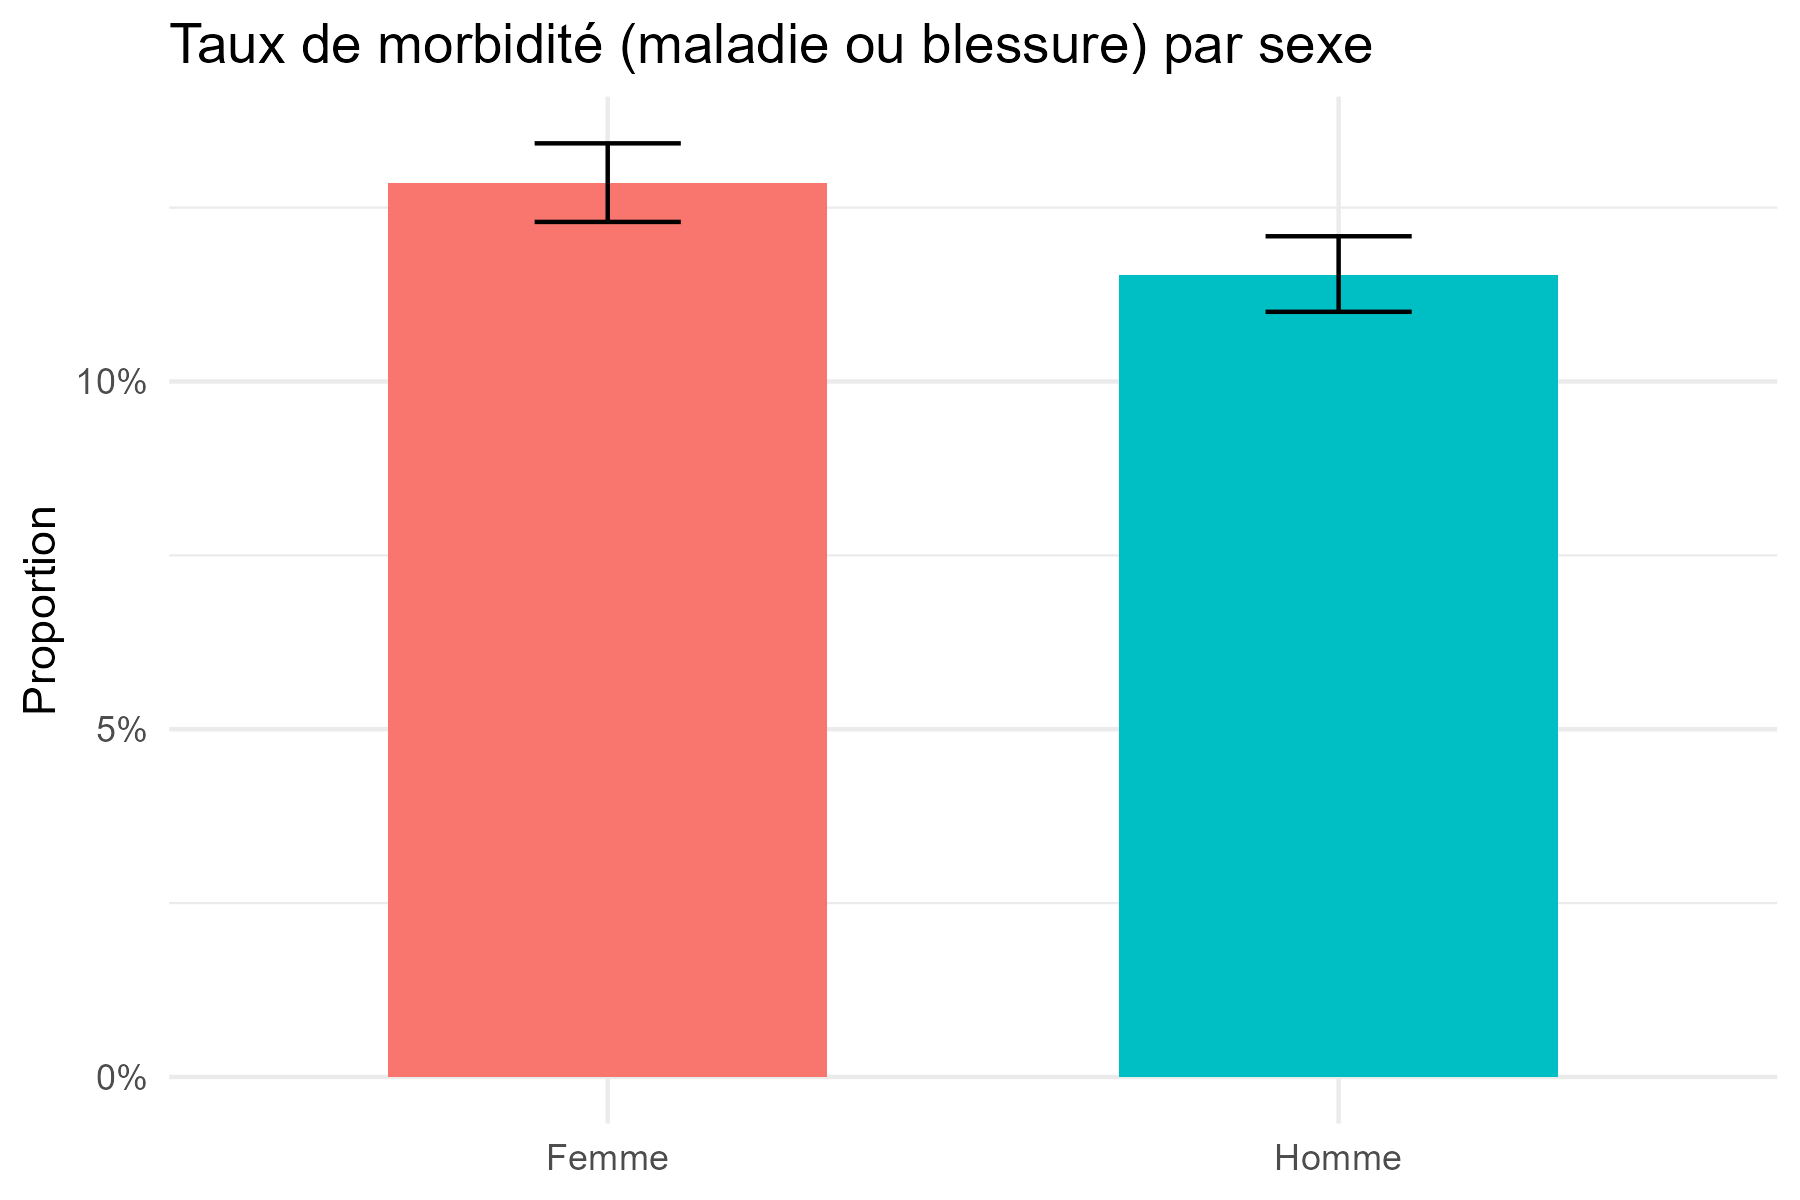
\includegraphics[width=1\linewidth]{../outputs/graphs/taux_morbidite_par_sexe} \end{center}

\subsubsection{Par Groupe d'Âge}\label{par-groupe-duxe2ge}

La morbidité augmente fortement avec l'âge : de 7,2 \% chez les 15--30
ans à 30,1 \% chez les 61 ans et plus. Les enfants de moins de 15 ans
présentent un taux de 11,9 \%, proche de la moyenne nationale. Ce profil
suit une courbe en U caractéristique : la morbidité est élevée chez les
enfants (11,9 \%), atteint son minimum chez les jeunes adultes de 15 -
30 ans (7,2 \%), groupe généralement en meilleure santé, puis augmente
continûment avec l'âge pour culminer à 30,1 \% chez les 61 ans et plus,
reflétant l'accumulation des maladies chroniques et la détérioration
physiologique liée au vieillissement.

\begin{longtable}[]{@{}lrrrrr@{}}
\caption{Taux de morbidité par groupe d'âge}\tabularnewline
\toprule\noalign{}
age\_group & n & n\_cases & prop & ic\_low & ic\_high \\
\midrule\noalign{}
\endfirsthead
\toprule\noalign{}
age\_group & n & n\_cases & prop & ic\_low & ic\_high \\
\midrule\noalign{}
\endhead
\bottomrule\noalign{}
\endlastfoot
0-14 ans & 11517 & 1366 & 0.119 & 0.113 & 0.125 \\
15-30 ans & 7272 & 522 & 0.072 & 0.066 & 0.078 \\
31-45 ans & 3868 & 433 & 0.112 & 0.102 & 0.122 \\
46-60 ans & 2688 & 453 & 0.169 & 0.155 & 0.183 \\
61 ans et plus & 1777 & 535 & 0.301 & 0.280 & 0.323 \\
\end{longtable}

\begin{center}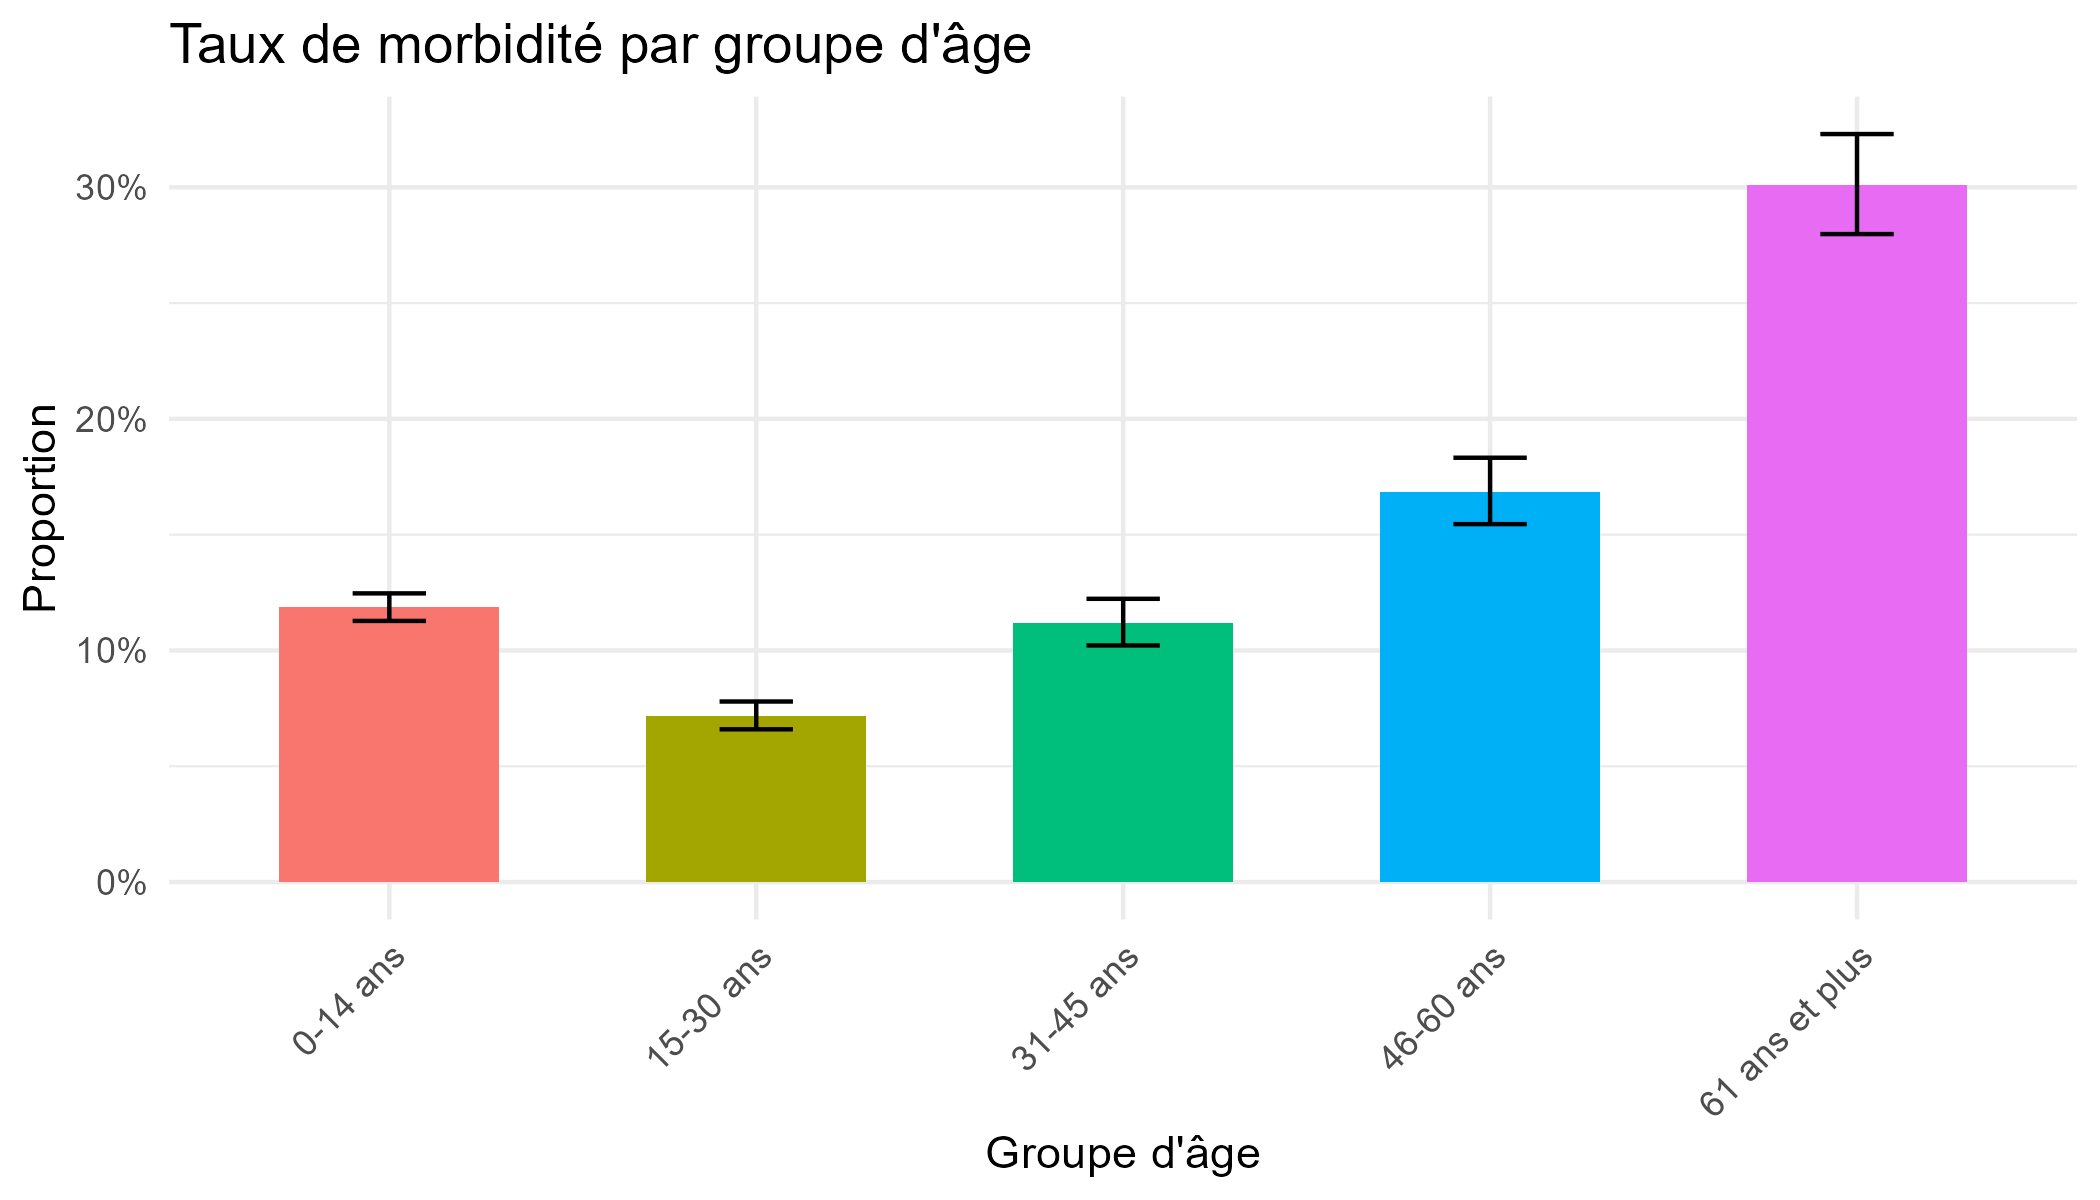
\includegraphics[width=1\linewidth]{../outputs/graphs/taux_morbidite_par_age} \end{center}

\subsection{Types de Problèmes de
Santé}\label{types-de-probluxe8mes-de-santuxe9}

Parmi les 3 309 individus ayant déclaré un problème, 94,0 \% ont
souffert d'une maladie, contre 6,0 \% d'une blessure.

\begin{longtable}[]{@{}lrrl@{}}
\caption{Répartition maladie vs blessure}\tabularnewline
\toprule\noalign{}
type & n & prop & prop\_label \\
\midrule\noalign{}
\endfirsthead
\toprule\noalign{}
type & n & prop & prop\_label \\
\midrule\noalign{}
\endhead
\bottomrule\noalign{}
\endlastfoot
Blessure & 198 & 0.06 & 6.0\% \\
Maladie & 3111 & 0.94 & 94.0\% \\
\end{longtable}

\subsection{Motifs de Consultation}\label{motifs-de-consultation}

L'analyse porte sur les 2 865 individus ayant consulté un professionnel
de santé. Le motif le plus fréquent est la maladie aiguë (52,4 \%),
suivi des check-up préventifs (20,5 \%) et du suivi de maladie chronique
(15,1 \%). Les blessures ne représentent que 4,1 \% des consultations.

\begin{longtable}[]{@{}lrr@{}}
\caption{Motifs de consultation (4 dernières semaines)}\tabularnewline
\toprule\noalign{}
motif\_lib & effectif & proportion \\
\midrule\noalign{}
\endfirsthead
\toprule\noalign{}
motif\_lib & effectif & proportion \\
\midrule\noalign{}
\endhead
\bottomrule\noalign{}
\endlastfoot
Maladie aiguë & 1502 & 0.524 \\
Check-up / préventif & 588 & 0.205 \\
Suivi maladie chronique & 433 & 0.151 \\
Blessure & 118 & 0.041 \\
Autre & 113 & 0.039 \\
Consultation prénatale & 61 & 0.021 \\
Suivi accident & 29 & 0.010 \\
Accouchement & 21 & 0.007 \\
\end{longtable}

\begin{center}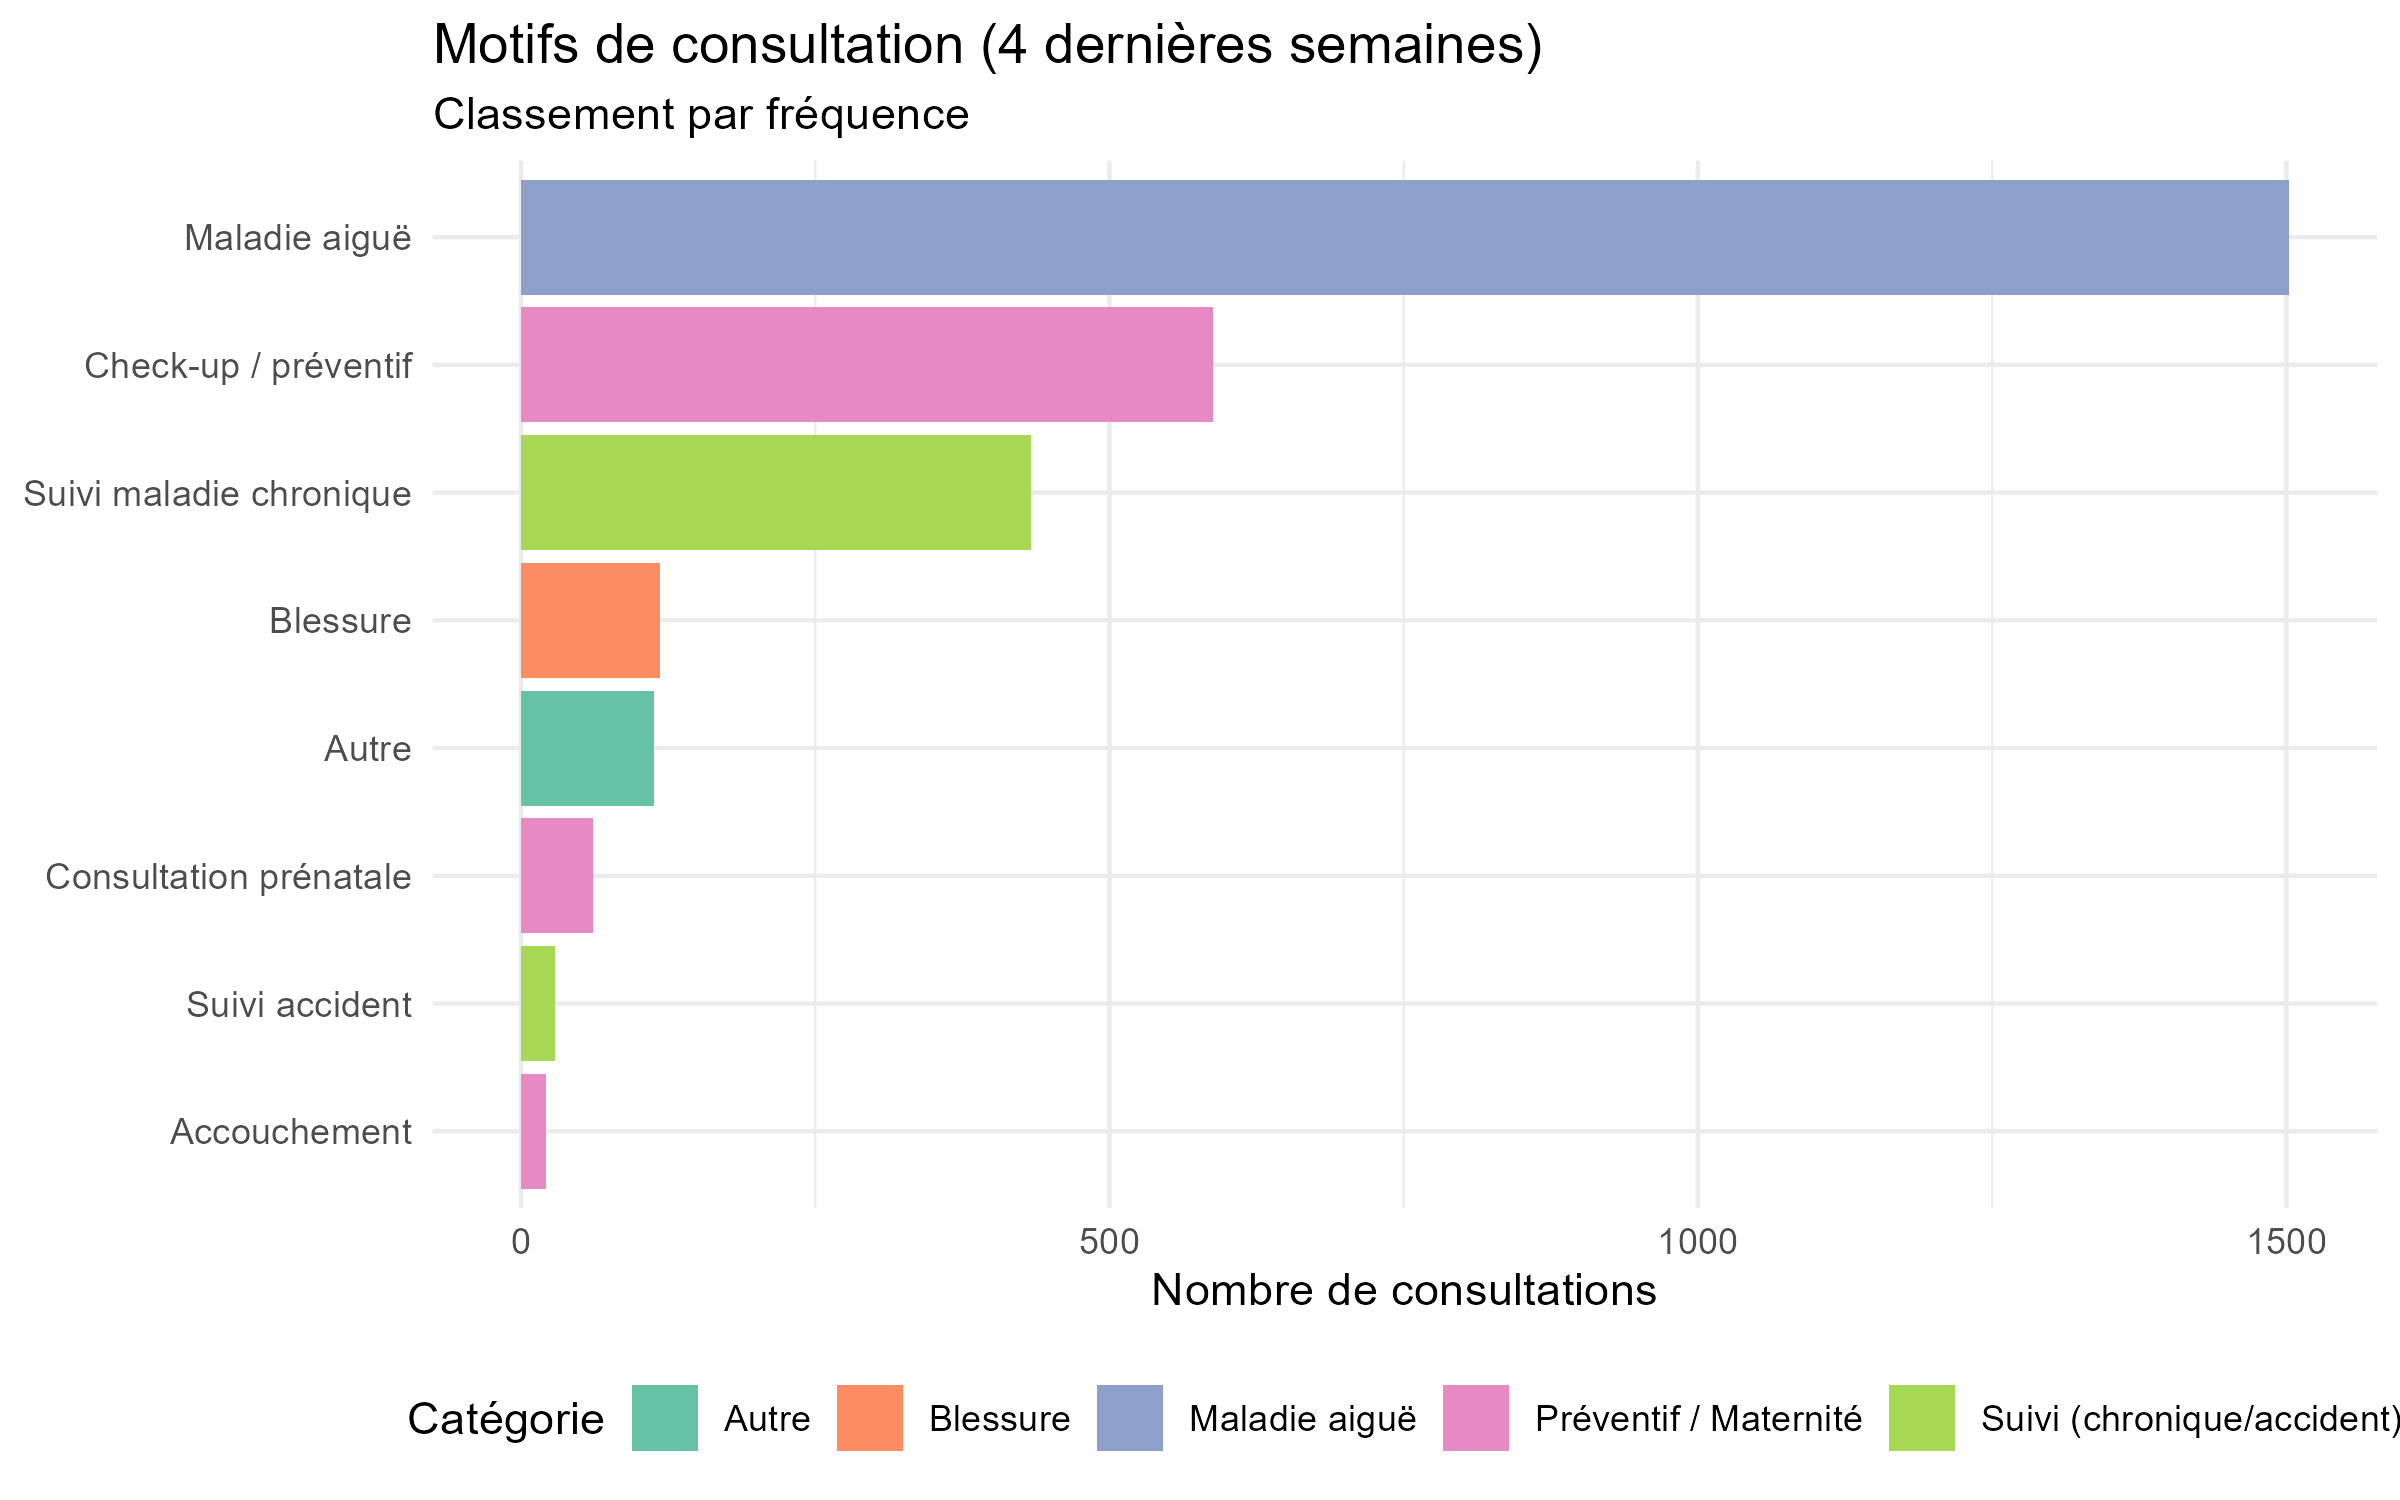
\includegraphics[width=1\linewidth]{../outputs/graphs/motifs_consultation_top10} \end{center}

\subsection{Recours aux Soins -- Type de
Prestataire}\label{recours-aux-soins-type-de-prestataire}

Le premier prestataire consulté est majoritairement un professionnel de
santé moderne : 47,8 \% des malades ont vu un médecin, infirmier ou
sage-femme. Les pharmacies et vendeurs de médicaments sont le second
recours (37,4 \%), tandis que les tradipraticiens sont consultés par
10,4 \% des individus. Seuls 1,7 \% déclarent n'avoir consulté personne.
Le recours massif aux pharmacies en premier lieu (37,4 \%) suggère une
automédication largement répandue au Nigeria, comportement courant en
Afrique subsaharienne qui mérite attention dans une perspective de santé
publique.

\begin{longtable}[]{@{}lrl@{}}
\caption{Type de prestataire consulté (premier recours)}\tabularnewline
\toprule\noalign{}
prestataire & n & prop\_label \\
\midrule\noalign{}
\endfirsthead
\toprule\noalign{}
prestataire & n & prop\_label \\
\midrule\noalign{}
\endhead
\bottomrule\noalign{}
\endlastfoot
Médecin / infirmier / sage-femme & 1583 & 47.8\% \\
Pharmacie / vendeur de médicaments & 1239 & 37.4\% \\
Tradipraticien / guérisseur & 345 & 10.4\% \\
Non renseigné & 77 & 2.3\% \\
Aucun & 56 & 1.7\% \\
Autre & 9 & 0.3\% \\
\end{longtable}

\begin{center}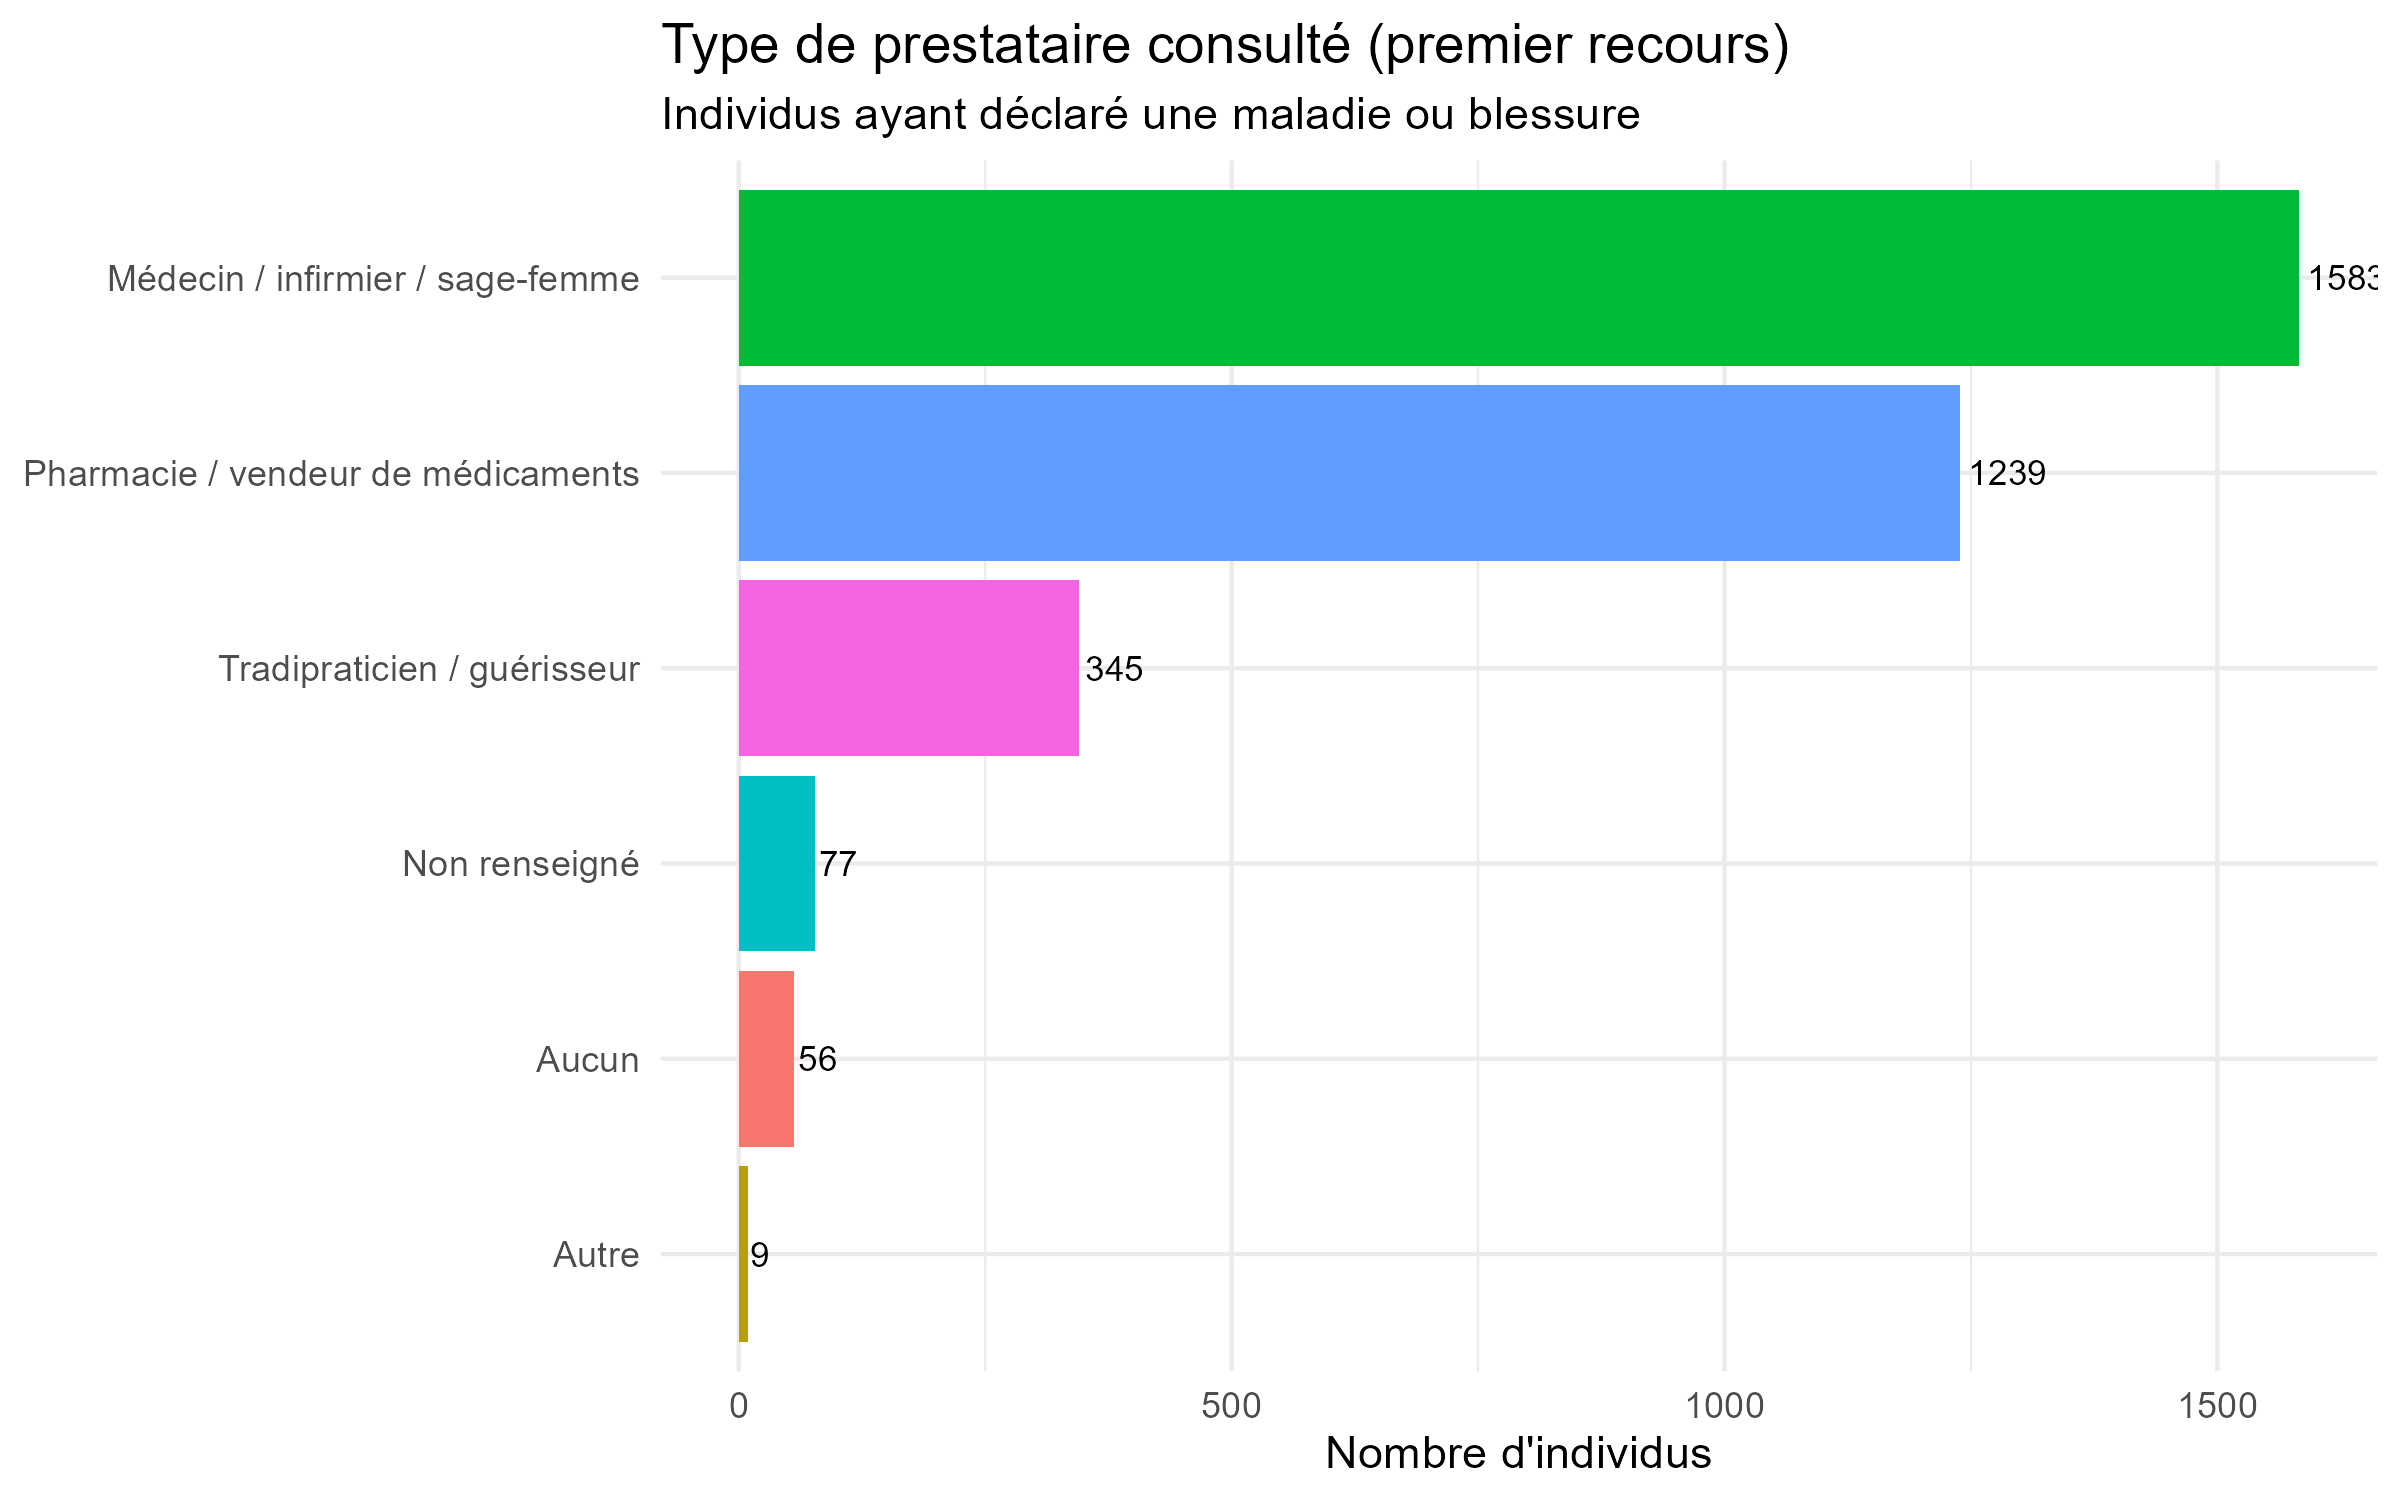
\includegraphics[width=1\linewidth]{../outputs/graphs/recours_soins_prestataire} \end{center}

\subsection{Dépenses de Santé}\label{duxe9penses-de-santuxe9}

\subsubsection{Distribution Générale}\label{distribution-guxe9nuxe9rale}

Les dépenses de santé sont très concentrées : la moyenne (8 090 Naira)
est bien supérieure à la médiane (2 500 Naira). Le tableau des déciles
montre que 10 \% des malades n'ont aucune dépense, tandis que 10 \%
dépensent plus de 15 000 Naira.

\begin{longtable}[]{@{}rrrrrrr@{}}
\caption{Statistiques globales des dépenses de santé}\tabularnewline
\toprule\noalign{}
mean & sd & median & Q1 & Q3 & min & max \\
\midrule\noalign{}
\endfirsthead
\toprule\noalign{}
mean & sd & median & Q1 & Q3 & min & max \\
\midrule\noalign{}
\endhead
\bottomrule\noalign{}
\endlastfoot
8090 & 25037 & 2500 & 980 & 6000 & 0 & 645000 \\
\end{longtable}

\begin{longtable}[]{@{}lr@{}}
\caption{Déciles des dépenses de santé}\tabularnewline
\toprule\noalign{}
decile & valeur \\
\midrule\noalign{}
\endfirsthead
\toprule\noalign{}
decile & valeur \\
\midrule\noalign{}
\endhead
\bottomrule\noalign{}
\endlastfoot
0\% & 0 \\
10\% & 350 \\
20\% & 700 \\
30\% & 1200 \\
40\% & 1700 \\
50\% & 2500 \\
60\% & 3500 \\
70\% & 4900 \\
80\% & 7500 \\
90\% & 15000 \\
100\% & 645000 \\
\end{longtable}

\begin{center}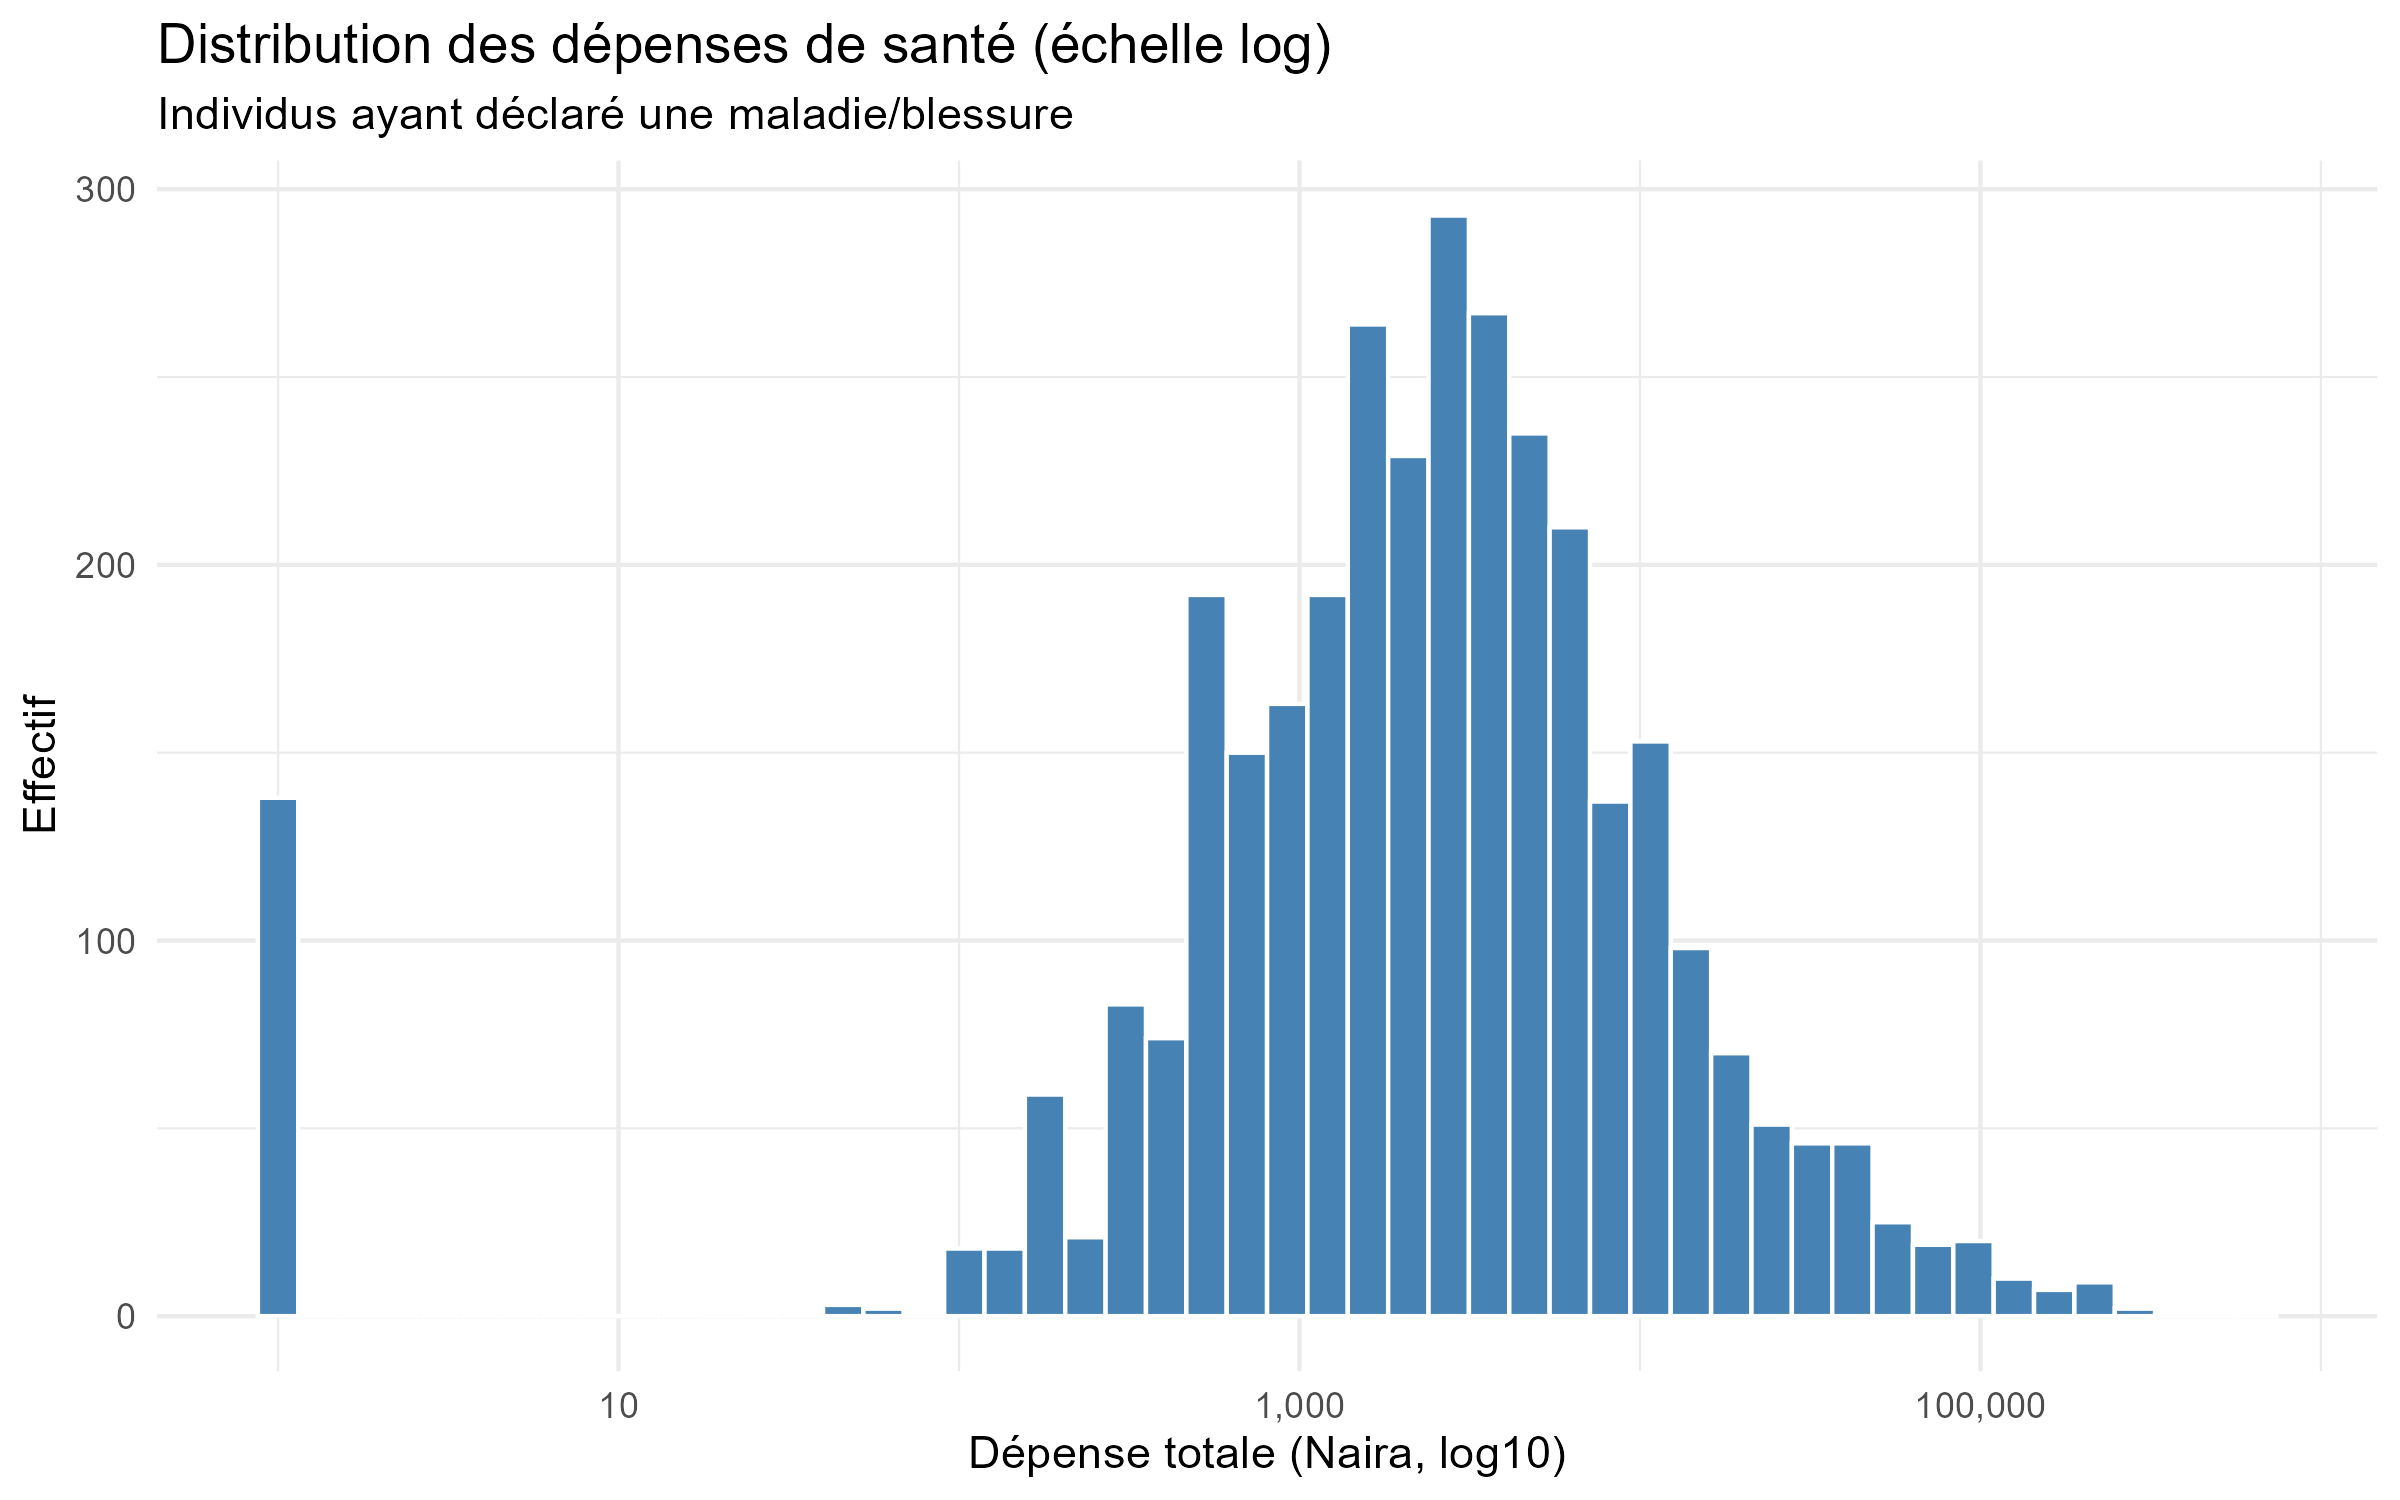
\includegraphics[width=1\linewidth]{../outputs/graphs/hist_depenses_sante_log} \end{center}

\subsubsection{Dépenses selon le
Prestataire}\label{duxe9penses-selon-le-prestataire}

Le boxplot ci-dessous compare les dépenses totales (échelle log) en
fonction du premier prestataire consulté. Les individus ayant consulté
un médecin ou une pharmacie ont des dépenses médianes plus élevées que
ceux ayant eu recours à un tradipraticien. La catégorie « Aucun » a la
dépense médiane la plus faible.

\begin{center}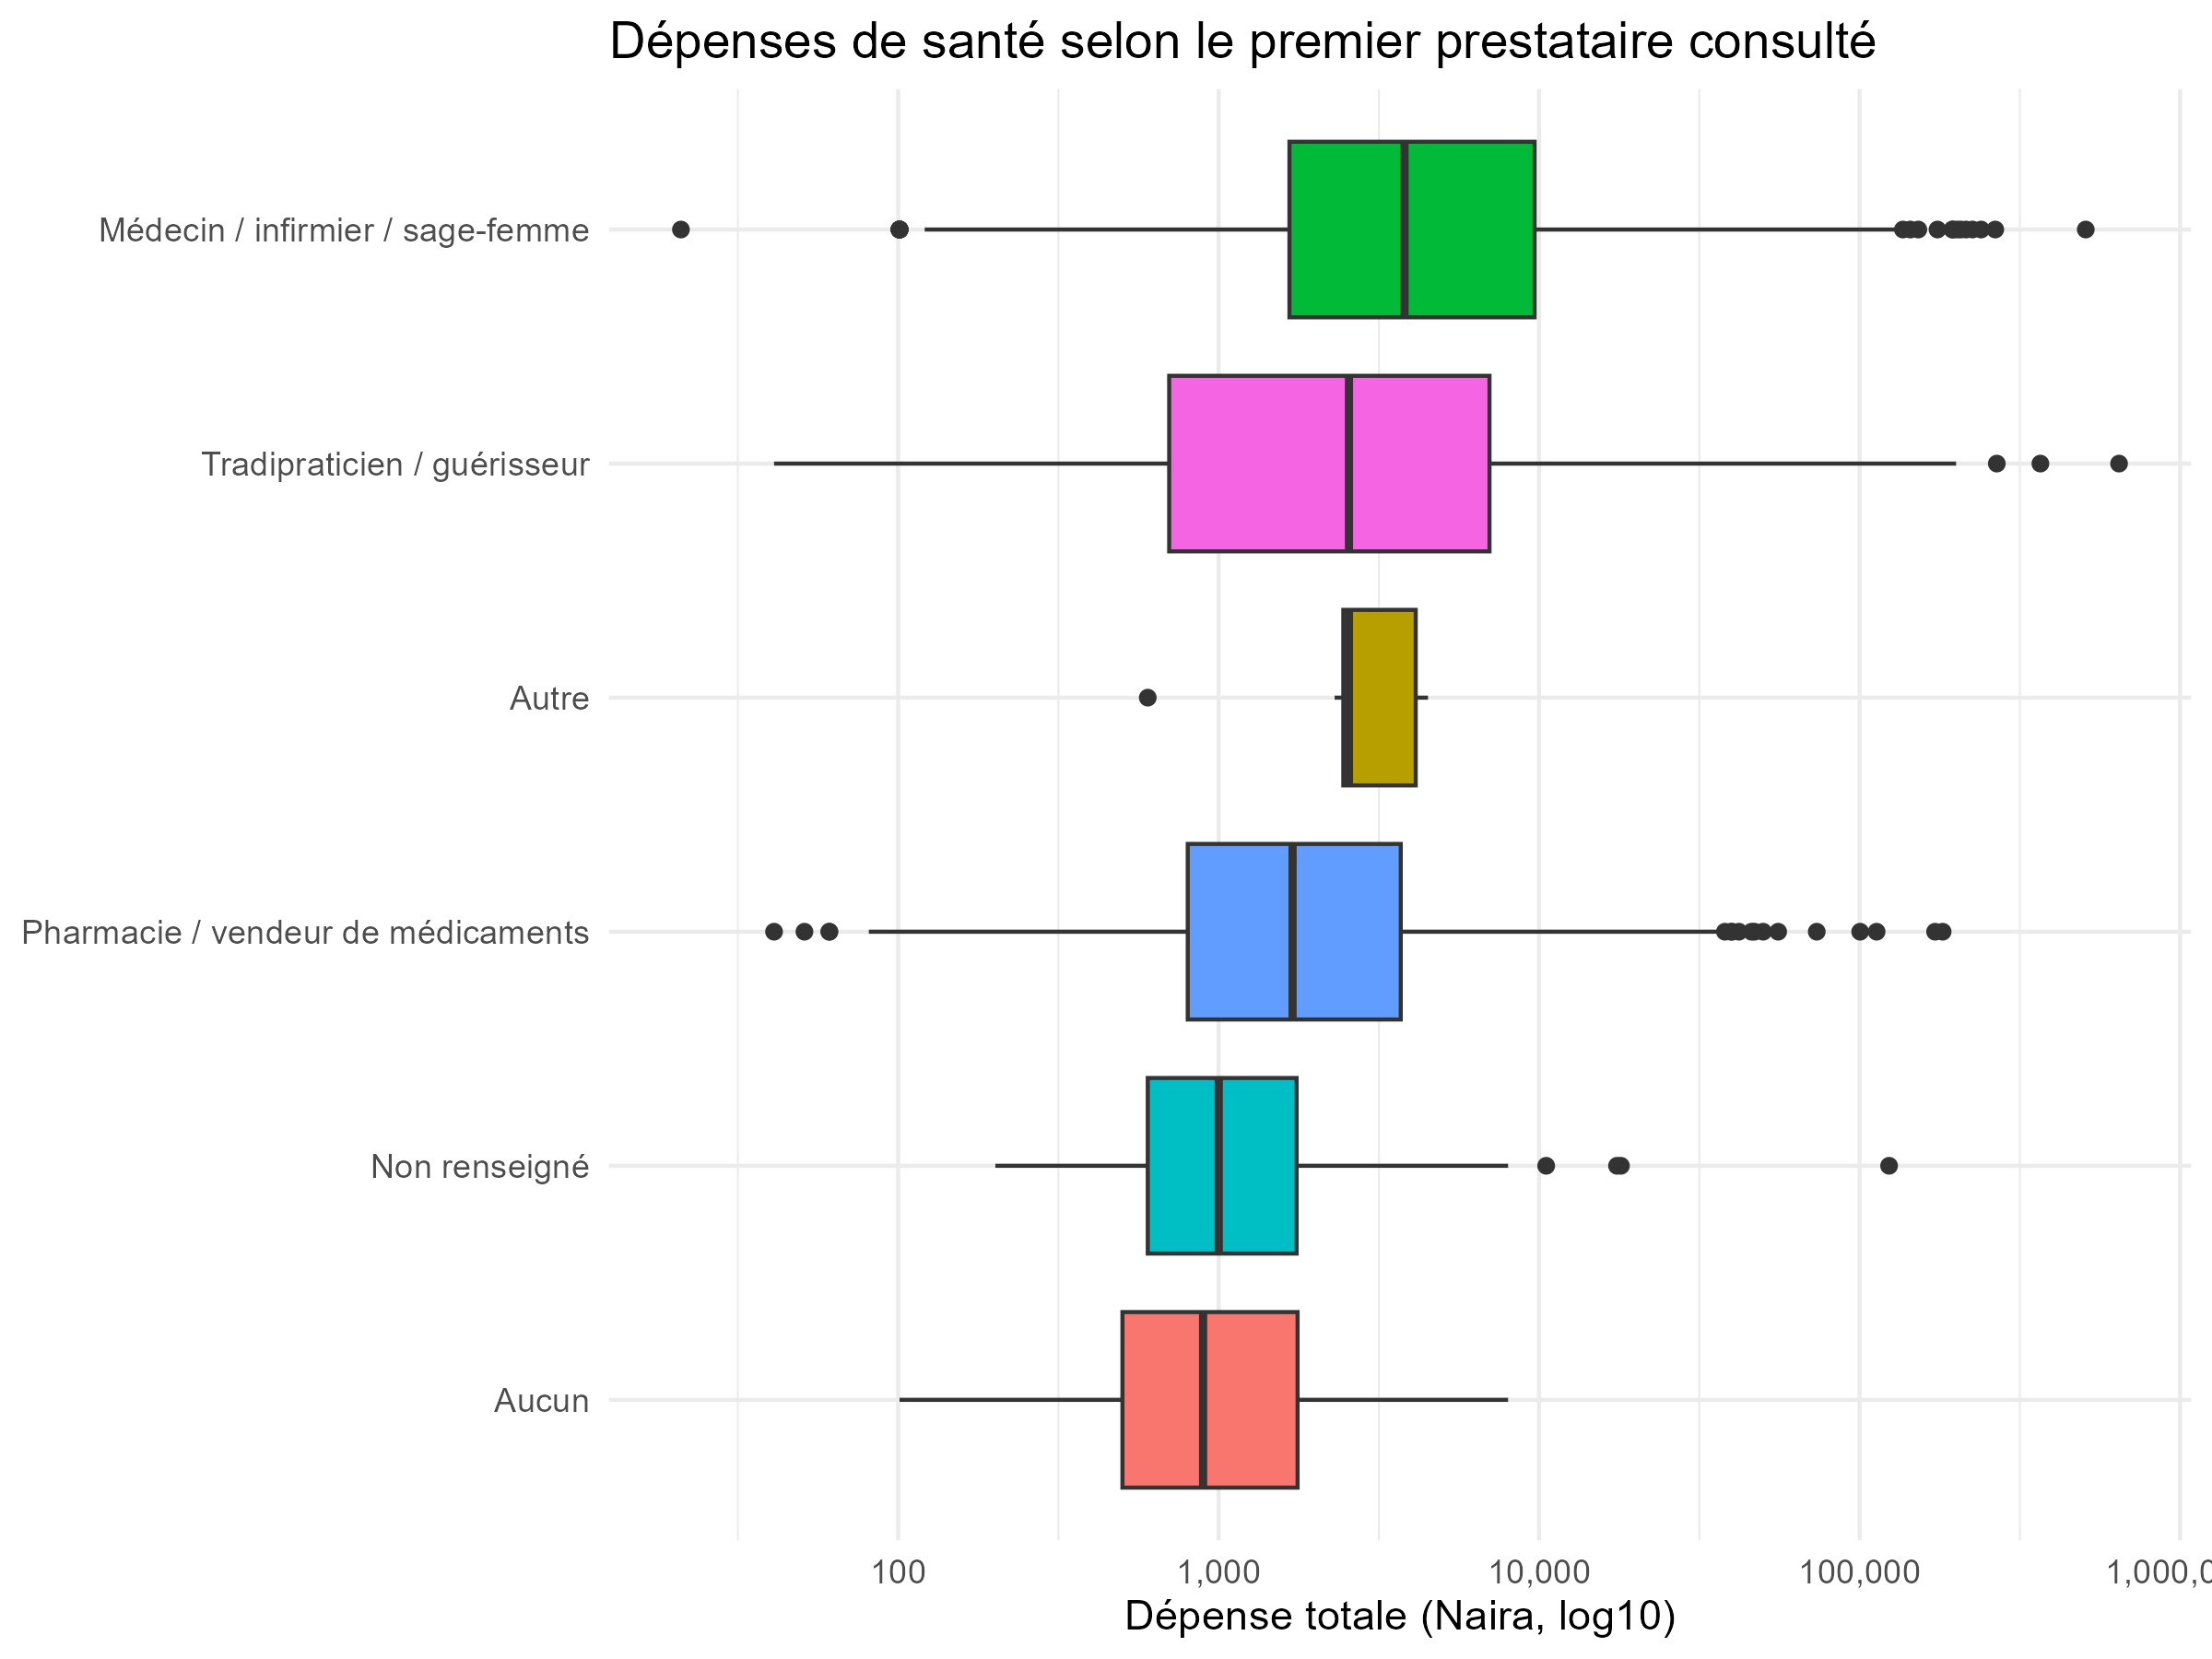
\includegraphics[width=1\linewidth]{../outputs/graphs/boxplot_depenses_par_prestataire} \end{center}

\subsubsection{Outliers}\label{outliers}

En appliquant la règle de l'écart interquartile (seuil à Q3 + 3 × IQR),
on identifie 240 individus (soit environ 7,3 \% des malades) comme des
outliers extrêmes, avec des dépenses supérieures à la borne de 21 060
Naira. La borne est calculée comme suit :

\[\text{borne} = Q_3 + 3 \times IQR = 6\,000 + 3 \times 5\,020 \approx 21\,060 \text{ Naira}\]

Ces cas correspondent à des hospitalisations coûteuses ou à des achats
importants de médicaments.

\subsection{Recours aux Soins et Niveau de
Vie}\label{recours-aux-soins-et-niveau-de-vie}

Le tableau de contingence croise la variable « a consulté » (0/1) avec
les quintiles de consommation (1 = plus pauvre, 5 = plus riche).

\begin{longtable}[]{@{}lrr@{}}
\caption{Recours aux soins selon le quintile de
consommation}\tabularnewline
\toprule\noalign{}
& Non consulté & Consulté \\
\midrule\noalign{}
\endfirsthead
\toprule\noalign{}
& Non consulté & Consulté \\
\midrule\noalign{}
\endhead
\bottomrule\noalign{}
\endlastfoot
Quintile 1 & 21 & 629 \\
Quintile 2 & 20 & 660 \\
Quintile 3 & 29 & 697 \\
Quintile 4 & 21 & 630 \\
Quintile 5 & 40 & 552 \\
\end{longtable}

Le test du \(\chi^2\) est significatif (p = 0,0033), indiquant une
dépendance entre le niveau de vie et le recours aux soins. Le V de
Cramér (0,069) témoigne toutefois d'une association faible.

Le graphique en barres 100 \% empilées montre que, dans tous les
quintiles, la très grande majorité des malades consulte (au moins 93
\%). On observe une légère baisse de la proportion de consultants chez
les plus riches (quintile 5 : 93,2 \% contre 96,8 \% dans les autres
quintiles).

\begin{center}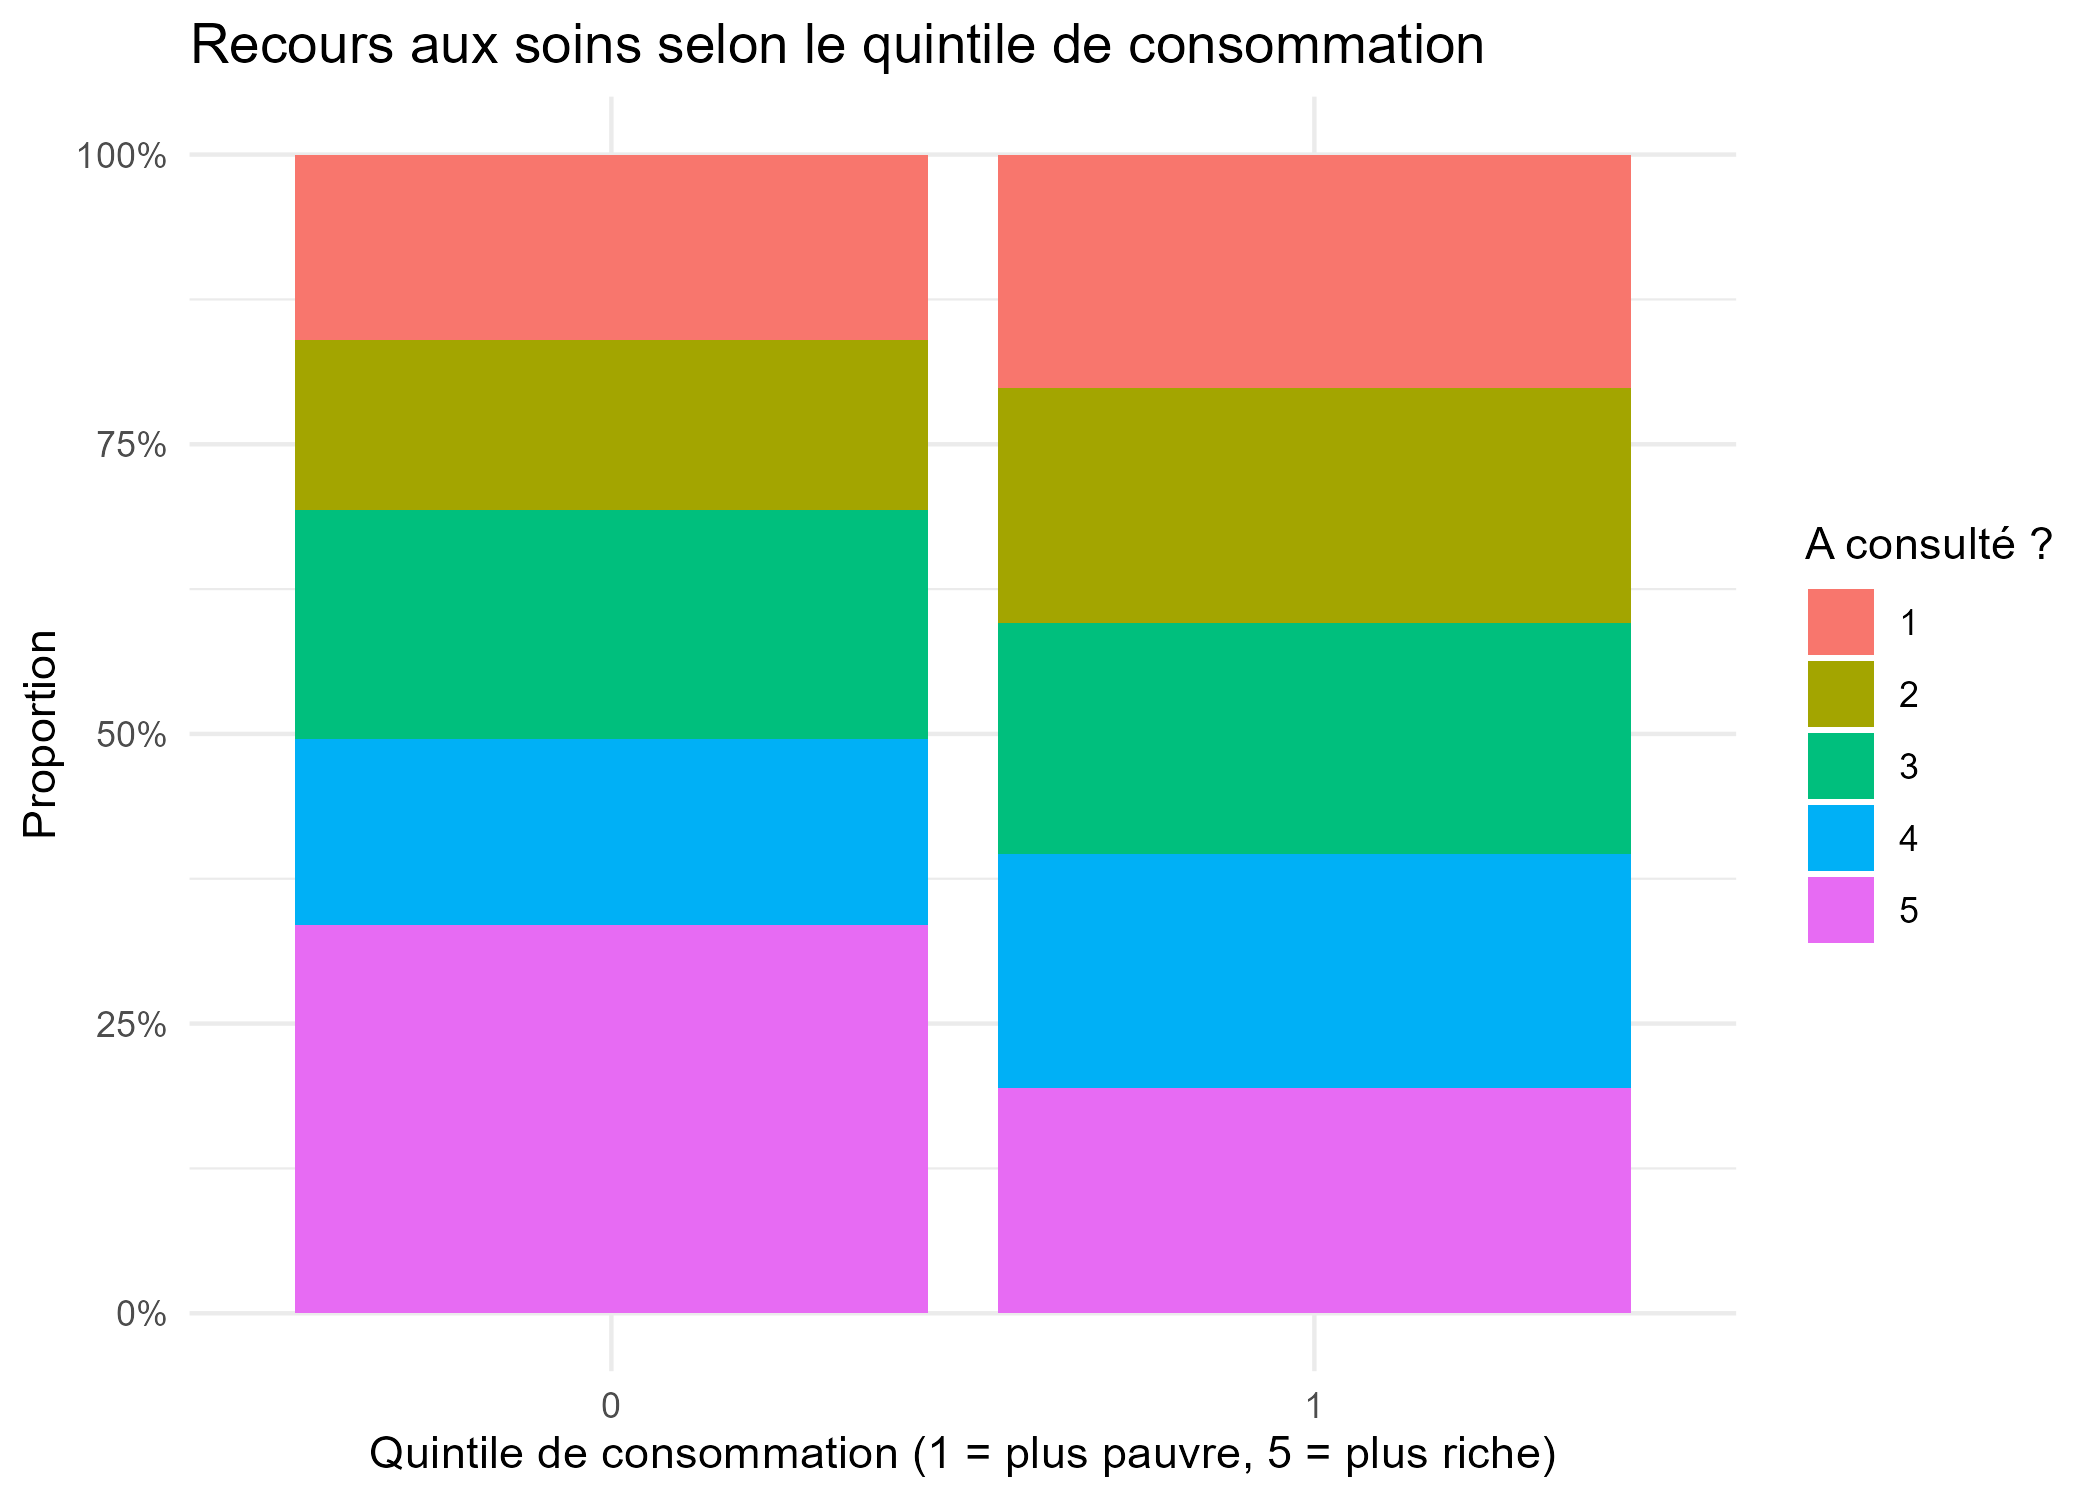
\includegraphics[width=1\linewidth]{../outputs/graphs/recours_soins_par_quintile} \end{center}

Ce résultat contre-intuitif (les ménages du quintile 5 consultent moins
fréquemment (93,2 \%) que ceux des quintiles inférieurs (96,8 \%)) peut
s'expliquer par une plus grande propension à l'automédication chez les
ménages aisés, une sous-déclaration des problèmes bénins, ou le recours
à des structures privées non captées par l'enquête.

\subsection{Comparaison Rural / Urbain des
Dépenses}\label{comparaison-rural-urbain-des-duxe9penses}

Les statistiques par milieu de résidence montrent des dépenses moyennes
plus élevées en milieu urbain (9 318 Naira) qu'en milieu rural (7 594
Naira). La médiane est également supérieure en ville (2 930 contre 2
325).

\begin{longtable}[]{@{}lrrrrrrrr@{}}
\caption{Dépenses de santé selon le milieu de résidence}\tabularnewline
\toprule\noalign{}
milieu & n & mean & median & sd & Q1 & Q3 & min & max \\
\midrule\noalign{}
\endfirsthead
\toprule\noalign{}
milieu & n & mean & median & sd & Q1 & Q3 & min & max \\
\midrule\noalign{}
\endhead
\bottomrule\noalign{}
\endlastfoot
Rural & 2356 & 7594 & 2325 & 23259 & 900 & 6000 & 0 & 645000 \\
Urbain & 953 & 9318 & 2930 & 28946 & 1050 & 6400 & 0 & 507800 \\
\end{longtable}

Le test de Wilcoxon confirme une différence significative (p = 0,0047).
Le violin plot ci-dessous illustre la distribution (échelle log) : les
urbains ont tendance à dépenser un peu plus, mais les deux groupes
présentent une forte variabilité et de nombreux outliers.

\begin{center}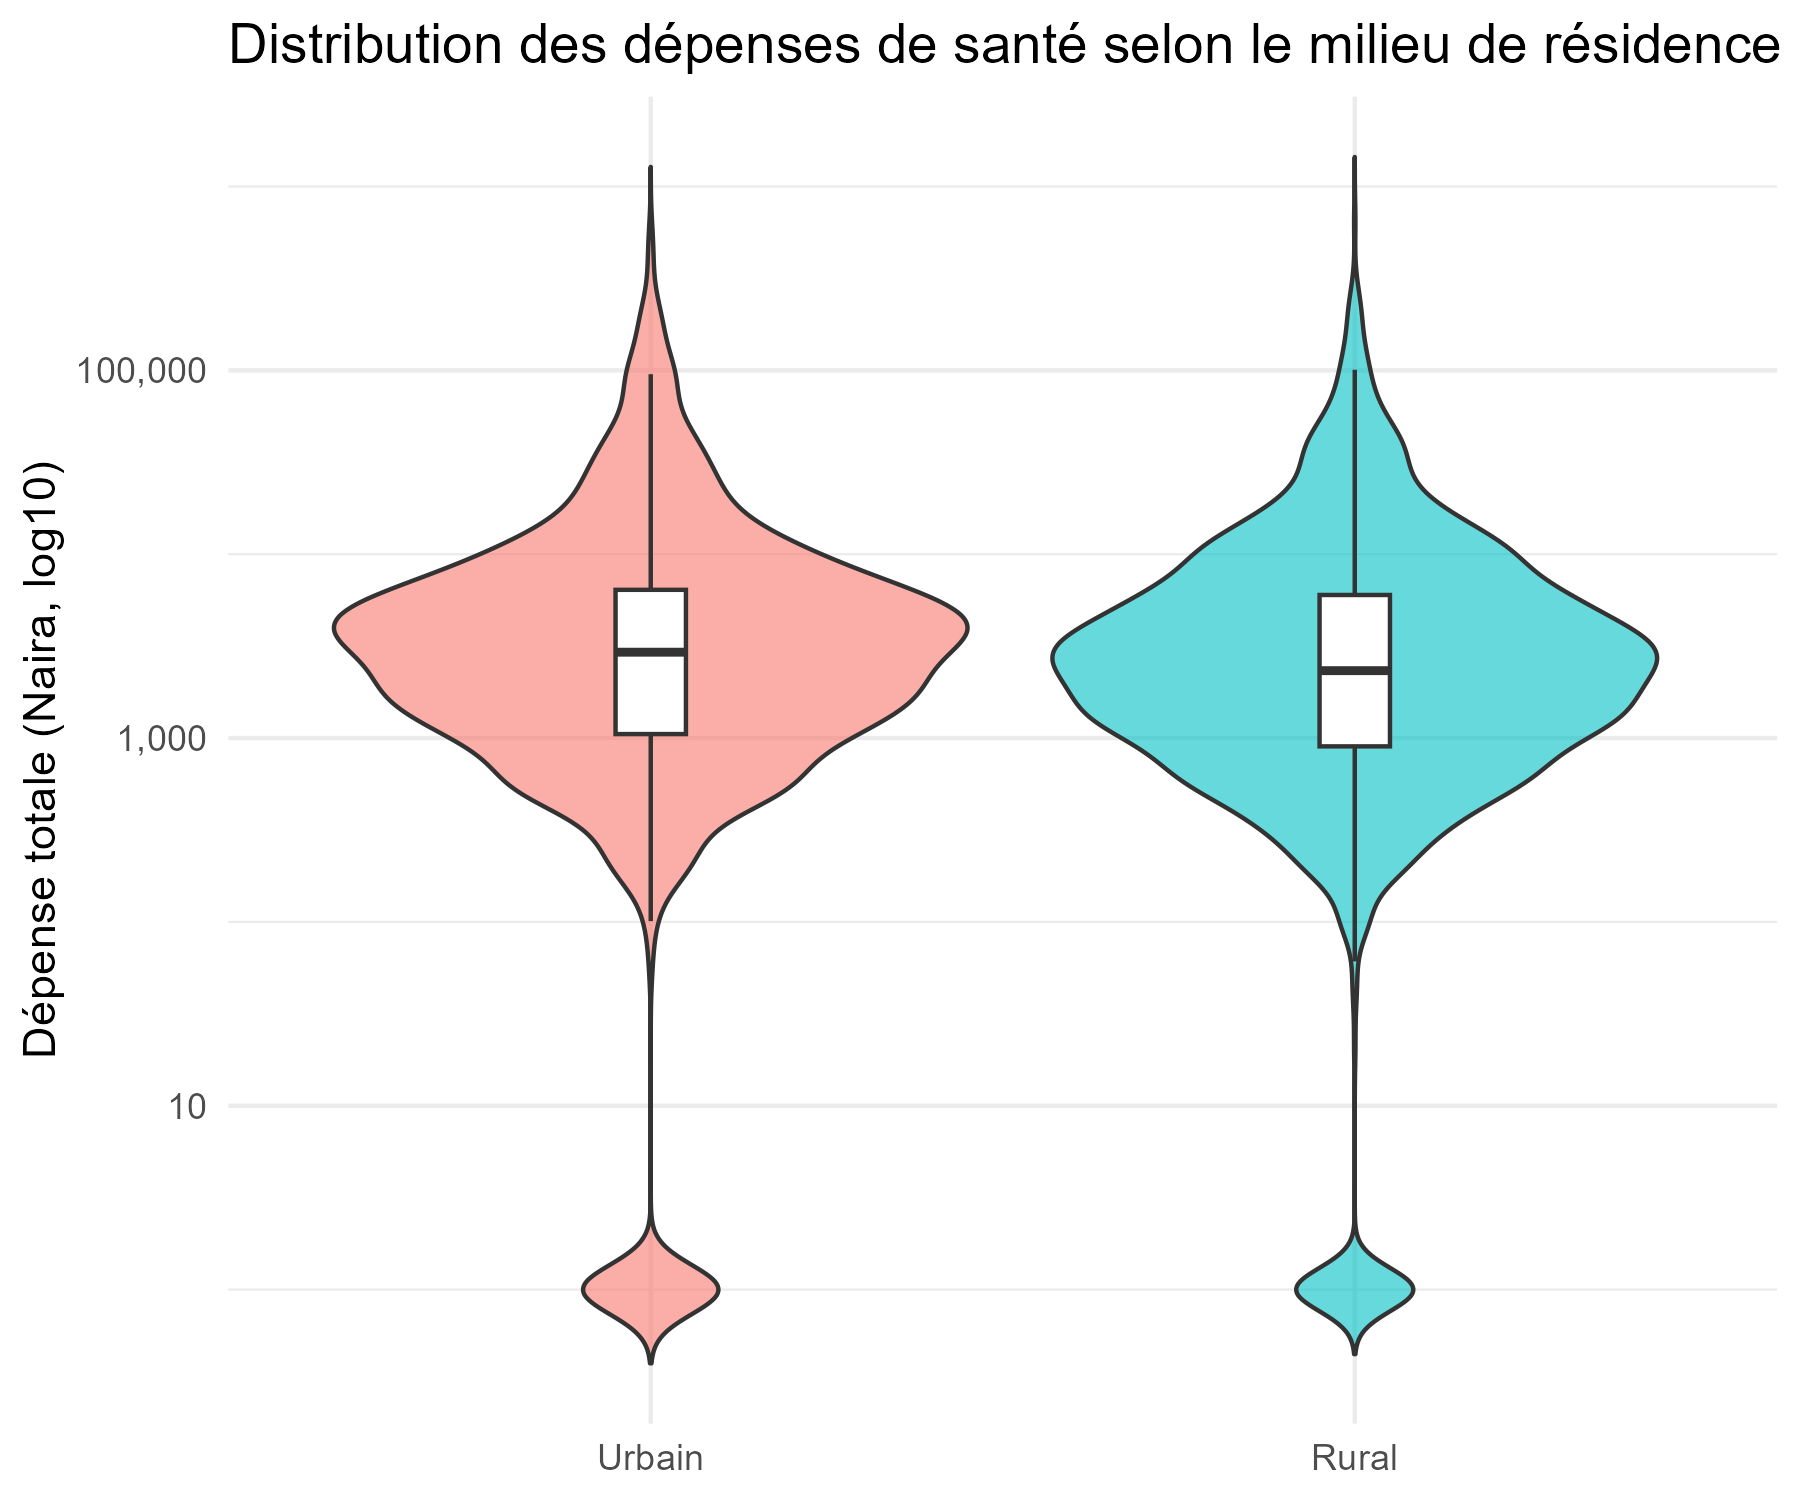
\includegraphics[width=1\linewidth]{../outputs/graphs/violin_depenses_rural_urbain} \end{center}

\section{Discussion}\label{discussion}

Les analyses confirment des disparités importantes dans la morbidité et
le recours aux soins :

\begin{itemize}
\item
  \textbf{Âge} : la morbidité augmente fortement après 60 ans,
  soulignant la vulnérabilité des personnes âgées.
\item
  \textbf{Sexe} : les femmes déclarent légèrement plus de problèmes de
  santé, ce qui peut refléter à la fois des différences biologiques et
  une plus grande propension à déclarer.
\item
  \textbf{Recours aux soins} : la quasi-totalité des malades consulte,
  principalement des professionnels de santé modernes. Le rôle des
  pharmacies et des tradipraticiens reste non négligeable.
\item
  \textbf{Dépenses} : très inégalitaires, avec une queue de distribution
  épaisse (outliers). Les dépenses sont significativement plus élevées
  en ville, peut-être en raison d'un accès à des soins plus coûteux ou
  d'une plus grande capacité à payer.
\item
  \textbf{Niveau de vie} : le lien avec le recours aux soins est
  statistiquement significatif mais faible ; les plus riches consultent
  même un peu moins souvent, ce qui pourrait s'expliquer par une
  automédication plus fréquente ou une moindre déclaration des problèmes
  bénins.
\end{itemize}

Au-delà des disparités quantitatives, ces résultats soulèvent la
question de l'équité dans l'accès aux soins de qualité. Si le taux de
recours est quasi universel (plus de 93 \% dans tous les quintiles), les
dépenses médianes restent faibles dans l'ensemble de la population (2
500 Naira), ce qui interroge sur la qualité et la complétude des soins
effectivement reçus, indépendamment du niveau de vie.

\textbf{Limites :}

\begin{itemize}
\item
  Les données ne permettent pas une classification fine des maladies
  (seulement maladie vs blessure). Nous avons utilisé les motifs de
  consultation comme proxy.
\item
  L'analyse des recours multiples (premier et second prestataire) n'a
  pas été réalisée ; elle pourrait affiner la compréhension des parcours
  de soins.
\item
  Les dépenses sont déclaratives et sujettes à des erreurs de mémoire.
\item
  Le niveau de vie est mesuré par la consommation totale, mais d'autres
  indicateurs (patrimoine, éducation) pourraient compléter l'analyse.
\end{itemize}

\section{Conclusion}\label{conclusion}

Ce travail a permis de décrire les principaux indicateurs de santé de la
population nigériane à partir de la vague 2 du GHS Panel. Il met en
évidence des inégalités de morbidité selon l'âge et le sexe, un recours
aux soins quasi systématique mais orienté vers différents types de
prestataires, et des dépenses de santé très concentrées, plus élevées en
milieu urbain. Le lien avec le niveau de vie, bien que significatif,
reste modeste.

Ces résultats constituent une base descriptive utile pour de futures
analyses plus approfondies (par exemple, sur les déterminants du
non-recours ou sur l'impact des dépenses de santé sur le bien-être des
ménages).

\end{document}
